%%%%%%%%%%%%%%%%%%%%%%%%%%%%%%%%%%%%%%%%%%%%%%%%%%%%%%%%%%%%%%%%%%%%%%%%%%%%%
%%%
%%% File: thesis.tex, version 0.1, May 2010
%%%
%%% =============================================
%%% This file contains a template that can be used with the package
%%% cs.sty and LaTeX2e to produce a thesis that meets the requirements
%%% of the Computer Science Department from the Technical University of Cluj-Napoca
%%%%%%%%%%%%%%%%%%%%%%%%%%%%%%%%%%%%%%%%%%%%%%%%%%%%%%%%%%%%%%%%%%%%%%%%%%%%%

\documentclass[12pt,a4paper,twoside,openright]{report}

\usepackage{cs}

% !!!!!!!!!!!!!!!!!!!!!!!!!!!! IMPORTANT NOTE !!!!!!!!!!!!!!!!!!!!!!!
% FOR THESIS IN ROMANIAN LANGUAGE COMMENT OUT THE FOLLOWING LINE !!!!
% FOR THESIS IN ENGLISH LANGUAGE COMMENT THE FOLLOWING LINE !!!!
\usepackage[english,romanian]{babel}


\graphicspath{{figures/}}
\ifpdf
  \DeclareGraphicsExtensions{.pdf,.jpeg,.png}
\else
  \DeclareGraphicsExtensions{.eps}
\fi

\mastersthesis
% \diplomathesis
% \leftchapter
% \centerchapter
% \rightchapter
\singlespace
% \oneandhalfspace
% \doublespace

\renewcommand{\thesisauthor}{Nume prenume student}    %% Your name.
\renewcommand{\thesismonth}{Iulie}     %% Your month of graduation.
\renewcommand{\thesisyear}{2016}      %% Your year of graduation.
\renewcommand{\thesistitle}{Titlul lucrării de disertație}

\renewcommand{\thesissupervisorname}{Titlul științific și numele cadrului diactic coordonator}


%\renewcommand{\thesisdedication}{To my beloved wife and parents}

\begin{document}


% ================================================================================
% ======================== FIRST TITLE PAGE =====================================
% ================================================================================

\begin{titlepage}

\thispagestyle{firststylewithoutfooter}

% \fancyhead{}
% \fancyhead[C]{
\includegraphics[width=20pt]{header-utcn-engleza.png}}
% \chead{
\includegraphics[width=20pt]{header-utcn-engleza.png}}


\begin{center}
% {\scshape \universitynameenglish} \\
% {\scshape \facultynameenglish} \\
% {\scshape \departmentnameenglish} \\

% {\scshape \universitynameromanian} \\
{\scshape \facultynameromanian} \\
{\scshape \departmentnameromanian} \\


\vspace{6cm}

\thesistitlesize {\textbf{\thesistitle}\\}
\vspace {1cm}

% \thesistypesize \textbf{\thesistypeenglish}\\
\Large \textbf{\thesistyperomanian}\\


\vspace{2cm}

% \thesisauthortypesize \thesisauthortypeenglish \\ \textbf{\thesisauthor} \\
\thesisauthortypesize \thesisauthortyperomanian \\ \textbf{\thesisauthor} \\

\vspace{1cm}

% \thesissupervisorsize \thesissupervisorenglish \\ \textbf{\thesissupervisorname}\\
\thesissupervisorsize \thesissupervisorromanian \\ \textbf{\thesissupervisorname}\\



\vspace{\stretch{1}}
{\thesismonth} {\thesisyear} \\
\end{center}
\end{titlepage}

\begin{titlepage}
\phantom{1}
\end{titlepage}


% ================================================================================
% ======================== SECOND TITLE PAGE =====================================
% ================================================================================

\begin{titlepage}

\begin{center}

\thispagestyle{firststylewithfooter}

% {\scshape \universitynameenglish} \\
% {\scshape \facultynameenglish} \\
% {\scshape \departmentnameenglish} \\

% {\scshape \universitynameromanian} \\
{\scshape \facultynameromanian} \\
{\scshape \departmentnameromanian} \\

\vspace{1cm}

\newcolumntype{R}{>{\raggedleft\arraybackslash}X}%
\begin{tabularx}{\textwidth}{lR}
% {\scshape \facultydeanenglish} & {\scshape \deptmanagerenglish} \\
{\scshape \facultydeanromanian} & {\scshape \deptmanagerromanian} \\
\facultydeanname & \deptmanagername\\
\end{tabularx}

\vspace {2cm}

\thesistitlesize {\textbf{\thesistitle}\\}
\vspace {1cm}

% \thesistypesize \textbf{\thesistypeenglish}\\
\thesistypesize \textbf{\thesistyperomanian}\\

\vspace{1cm}

\end{center}

% \vspace{1cm}

\begin{flushleft}
\begin{enumerate}
%   \item \textbf{\thesisauthortypeenglish}: \thesisauthor
  \item \thesisauthortyperomanian: \thesisauthor
 
%  \item \textbf{\thesissupervisorenglish}: \thesissupervisorname
 \item \thesissupervisorromanian: \thesissupervisorname
 
%  \item \textbf{\thesiscontentsenglish}: Thesis presentation, suprvisior evaluation, chapter 1, chapter 2, \dots, chapter n, References, Anexes, CD.
 \item \thesiscontentsromanian: Pagina de prezentare, aprecierile coordonatorului, titlul capitolului 1, titlul capitolului 2, \dots, titlul capitolului n, bibliografie, anexe, CD.
 
%  \item \textbf{\thesisworkingplaceenglish}: UTCN, Cluj-Napoca
 \item \thesisworkingplaceromanian: UTCN, Cluj-Napoca

%  \item \textbf{\thesisadvisorsenglish}: Donald Knuth, Leslie Lamport, others \dots
 \item \thesisadvisorsromanian: Donald Knuth, Leslie Lamport, others \dots

%  \item \textbf{\thesisbegindateenglish}: \dotfill
 \item \thesisbegindateromanian: \dotfill

%  \item \textbf{\thesisenddateenglish}: \dotfill
 \item \thesisenddateromanian: \dotfill

\end{enumerate}

\end{flushleft}

\vspace{0.5cm}

\begin{center}

\newcolumntype{R}{>{\raggedleft\arraybackslash}X}%
\begin{tabularx}{\textwidth}{lR}
% {\thesissignatureenglish} {\thesissupervisorenglish} & {\thesissignatureenglish} {\thesisauthortypeenglish} \\
{\thesissignatureromanian} {\thesissupervisorromanian} & {\thesissignatureromanian} {\thesisauthortyperomanian} \\
\thesissupervisorname & \thesisauthor \\
\end{tabularx}

\vspace{\stretch{1}}
{\thesismonth} {\thesisyear} \\

\end{center}

\end{titlepage}


\begin{titlepage}
\phantom{1}
\end{titlepage}


% ================================================================================
% ======================== THIRD TITLE PAGE =====================================
% ================================================================================

\begin{titlepage}

\begin{center}
\thispagestyle{firststylewithfooter}

% {\scshape \universitynameenglish} \\
% {\scshape \facultynameenglish} \\
% {\scshape \departmentnameenglish} \\

% {\scshape \universitynameromanian} \\
{\scshape \facultynameromanian} \\
{\scshape \departmentnameromanian} \\
\end{center}

\vspace{3cm}

\begin{center}
% \autheticitydeclarationsize \textbf{\autheticitydeclarationenglish}
\autheticitydeclarationsize \textbf{\autheticitydeclarationromanian}
\end{center}

\vspace{1cm}

Subsemnatul \textit{\thesisauthor}, legitimat cu \textit{CI/BI} seria \textit{XX} numărul \textit{NNNNNN}, CNP \textit{LLLLLLLLLLLL}, autorul lucrării \textit{\thesistitle} elaborată în vederea susținerii examenului de finalizare a studiilor de masterat la Facultatea de Automatică și Calculatoare, Departamentul Calculatoare, Specializarea \textit{SSSSSSSS} din cadrul Universității Tehnice din Cluj-Napoca, sesiunea \textit{\thesismonth} a anului univeristar \textit{20XX/20XX}, declar pe proprie răspundere, că această lucrare este rezultatul propriei mele activități intelectuale, pe baza cercetărilor mele și pe baza informatiilor obținute din surse care au fost citate în textul lucrării și în bibliografie.

Declar că această lucrare nu conține porțiuni plagiate, iar sursele bibliografice au fost folosite cu respectarea legislației române și a convențiilor internaționale privind drepturile de autor.

Declar, de asemenea, că această lucrare  nu a mai fost prezentată în fața unei alte comisii de examen de licență sau disertație.

În cazul constatării ulterioare a unor declarații false, voi suporta sancțiunile administrative, respectiv, \textit{anularea examenului de disertație}.


\vspace{2cm}

\begin{center}

\newcolumntype{R}{>{\raggedleft\arraybackslash}X}%
\begin{tabularx}{\textwidth}{lR}
% Cluj-Napoca & {\thesissignatureenglish{ }\thesisauthortypeenglish}\\
% date  & {\thesisauthor} \\
Cluj-Napoca & {\thesissignatureromanian}\\
data  & {\thesisauthortyperomanian} \\ 
\end{tabularx}

\end{center}


\end{titlepage}


\begin{titlepage}
\phantom{1}
\end{titlepage}


%\pagestyle{headings}

% ABSTRACT
\begin{abstract}
Descrierea sumară a lucrării, în câteva fraze. Un site foarte util ce conține exemple \LaTeX se găsește la \url{http://en.wikibooks.org/wiki/LaTeX}.
Recomandăm crearea unui proiect în editoare Latex specializate (exemplu Kile pe Linux, TexnicCenter pe Windows) astfel încât compilarea/translatarea codului Latex în PDF să se facă din orice fișier editați la un moment dat (practic se va compila proiectul). De asemenea, dacă fișierul ``thesis.bib'' este inclus în proiect, există facilitatea de code-completion și la cite. 
\end{abstract}

\begin{titlepage}
\phantom{1}
\end{titlepage}



%\thesistitle                    %% Generate the title page.
%\authordeclarationpage                %% Generate the declaration page.

\pagenumbering{roman}
\setcounter{page}{1}

\tableofcontents
% \newpage

\listoftables

\listoffigures

% \clearpage
% \newpage

\begin{titlepage}
\phantom{1}
\end{titlepage}



\pagenumbering{arabic}
\setcounter{page}{1}

% \pagestyle{normalpagestyle}
% \pagestyle{fancy}
% \fancyhf{}

\setlength{\headheight}{15pt}

\pagestyle{fancy}
\renewcommand{\chaptermark}[1]{ \markboth{\thechapter. #1}{} }
\renewcommand{\sectionmark}[1]{ \markright{\thesection. #1}{} }

\renewcommand{\headrulewidth}{1pt} % remove lines as well
\renewcommand{\footrulewidth}{1pt}

% \renewcommand\footrule{
%   \begin{minipage}{1\textwidth}
%     \hrule width \hsize height 2pt \kern 1mm \hrule width \hsize   
%   \end{minipage}\par
% }%
% 
% \renewcommand\headrule
% {
%   \begin{minipage}{1\textwidth}
%     \hrule width \hsize \kern 1mm \hrule width \hsize height 2pt 
%   \end{minipage}
% }%


\fancyhf{}
% \fancyhead[LE,RO]{\thepage}
\fancyhead[LE]{\textit{ \nouppercase{\leftmark}} }
\fancyhead[RO]{\textit{ \nouppercase{\rightmark}} }
\fancyfoot[RE]{{\thesismonth} {\thesisyear}}
% \fancyfoot[LE,RO]{Page \thepage\ of \pageref{LastPage}}
\fancyfoot[LE,RO]{\thepage}

\fancypagestyle{plain}{ %
  \fancyhf{} % remove everything
%   \renewcommand\footrule{}
%   \renewcommand\headrule{}
  \renewcommand{\headrulewidth}{0pt} % remove lines as well
  \renewcommand{\footrulewidth}{1pt}
%   \fancyfoot[LE,RO]{Page \thepage\ of \pageref{LastPage}}
  \fancyfoot[LE,RO]{\thepage}
}




% \chapter{Introduction}
\chapter{Introducere}
\label{cap:Introducere}
 \section{Contextul lucrării}
if abcdneeded in this chapter i could write about how tradiitional cnn was enhanced to be able to detect and segment \newline
Conform statisticilor Poliției Române \cite{politia_romana}  în anul 2017 în România au fost 8624 de accidente rutiere în care 1951 oameni și-au pierdut viața iar 8172 oameni au fost răniți grav. Dacă ne uităm pe statiscticile întregii lumi \cite{WHO}  vedem că cca. 1,3 milioane de oameni mor anual în accidente rutiere.\newline
Statisticile de accidente ne arată că  în 94\% dintre toate accidentele are rol și eroarea umană, iar 76\% sunt cauzate numai de eroarea umană.
 Fred Wegman și Letty Aarts  în \cite{SWOV} prezintă că în accidentele rutiere cei mai vulnerabili sunt pietonii (în special copiii) și bicicliștii aceștia fiind neprotejați. Locul doi pe lista de top a vulnerabilității o țin conducătorii de motociclete, mopeduri, etc. pentru că ei sunt numai parțial protejați (\ref{fig:lethalities}).\newline

%image of table with vulnerabilities in age and transport modes categories
\begin{figure}[h!]
    	\centering
	\captionsetup{justification=centering, margin=2cm}
	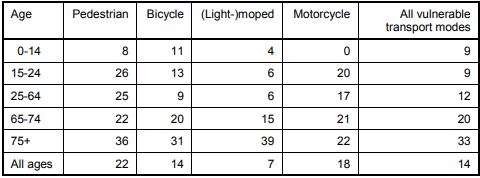
\includegraphics[width=0.8\textwidth]{figures/lethality_rates.png}
	\caption{Numărul de persoane implicate separate după vârstă și modul de transport pe 100 accidente serioase \cite{SWOV}}
	\label{fig:lethalities}
\end{figure}

Numerele acestea ridicate motivează aspirația noastră spre a construi sisteme inteligente care pot ne să ajute la evitarea dramelor rutiere. Avem două așteptări cruciale față de un asemenea sistem inteligent: să funcționeze în timp real și să aibă o rată foarte ridicată de detecție corectă. Alarmele false sunt costisitoare și iritante pentru persoanele aflate în vehicul, iar greșelile în care sistemul nu recunoaște pericolul pot avea consecințe fatale.\newline
Pentru luarea deciziilor, sistemul trebuie să obțină informațiile necesare din scenele de trafic, iar acest lucru se poate face prin mai multe modalități; în \cite{car_sensors}  Gert Rudolph și Uwe Voelzke prezintă cele mai folosite metode de colectarea informațiilor pentru mașini autonome:
\begin{itemize}
	\item Camere video 360$^\circ$: fără îndoială imaginile video conțin peste 90\% din informația de care are nevoie un conducător uman dar sunt potrivite și pentru conducerea vehiculelor autonome. Este critic ca camerele folosite să se descurce în toate condițiile de luminare și stare atmosferică.
	\item Radio Detection And Ranging (RADAR): sistemele ADAS (Advanced Driver Assistance Systems) necesită un număr mare de senzori, aceștia facând o contribuție la conducerea autonomă. RADARele se folosesc în asistarea parcării, în recunoașterea situațiilor în care este nevoie de frânare imediată, măsurarea distanțelor, etc.
	\item Light Detection And Ranging (LiDAR): LiDAR este un sistem bazat pe laser, relativ nou în contextul vehiculelor autonome. Pe lângă \textit{transmitter} (laser) este nevoie și de un \textit{receiver} foarte sensibil. Folosit în primul rând pentru măsurarea distanțelor obiectelor staționare și a celor în mișcare, sistemul folosește proceduri speciale pentru construirea unei imagini 3D a obiectelor detectate.
	\item Sonare ultrasonice, GPS, senzori termale, etc.
\end{itemize}
Deși pentru oameni recunoașterea actorilor dintr-o scenă de trafic este o problemă trivială, pentru sistemele informatice este una dificilă, aceștia având nevoie de algoritmi isteți. Condițiile de luminare, vizibilitate precum și trăsăturile obiectelor (rotație, mărime, mișcare, culorile, etc.) sunt factori care îngreunează recunoașterea actorilor dintr-o scenă.

\section {Tema Lucrării}
Tema lucrării de față este recunoașterea actorilor în imaginile captate din scene de trafic urban folosind inteligență artificială. Astfel se află la intersecția a două domenii care au primit foarte multă atenție recent: viziune artificială și inteligență artificială; cu algoritmi de procesare de imagini se vor extrage informații din imagini, iar cu ajutorul unei rețele neuronale se va face detectarea obiectelor în imaginile prelucrate precum și segmentarea semantică a imaginilor.\newline
De ce rețelele neuronale (convoluționale)? Putem să motivăm această decizie cu un mic exemplu luat din cadrul recunoașterii obiectelor dintr-o imagine: să propunem că problema noastră este de a face un program care poate recuoască un cub simplu, fără nicio textură specială pe o imagine. Chiar și acest obiect simplu introduce mii de probleme dacă folosim metode tradiționale: obiectul poate fi mai mic sau mai mare, se poate roti; și diferitele condiții de luminare pot să încurce programul nostru, precum și zgomotul din imagine. Și ce se întâmplă dacă vrem să recunoaștem un cub care poate să aibă și textură? Durere de cap! Am avea nevoie de o cantitate imensă de pre-procesări ca să putem să tragem concluzii uniforme.\newline
Aici intră în "imagine" puterea rețelelor neuronale. Acestea nu au nevoie de nicio trăsătură unică și specială care diferențiază o categorie de obiecte de o altă categorie. Dacă rețeaua neuronală are un set de antrenare variat și destul de mare, poate să tragă concluzii și să facă generalizări despre obiecte acestea fiind imune la zgomote; funcționând asemănător cu cortexul vizual animalelor, o rețea neuronală antrenată este greu de înșelat.\newline
Domeniul exact al temei este clasificarea imaginilor, detecția obiectelor și segmentarea semantică a imaginilor folosind rețele neuronale \textit{convoluționale}(CNN).
%image presenting image classification, detection and segmentation
\begin{figure}[h!]
    	\centering
	\captionsetup{justification=centering, margin=2cm}
	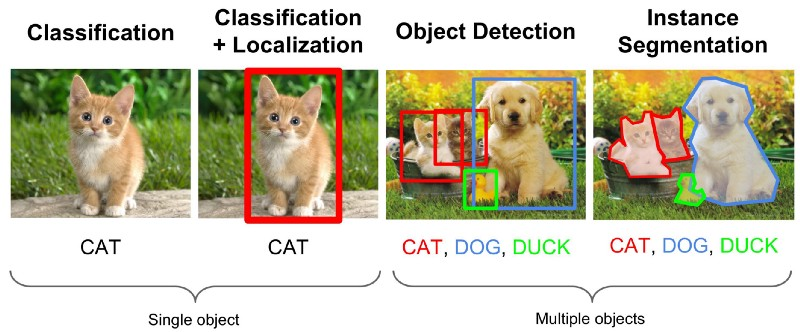
\includegraphics[width=0.9\textwidth]{figures/class_detect_segment.jpeg}
	\caption{Clasificare de imagine, localizare, detecție de obiecte, segmentare semantică \cite{class_detect_segment}}
	\label{fig:class_detect_semgent}
\end{figure}
Dacă ne uităm pe figura - putem să înțelegem ce înseamnă aceste concepte și că vorbim de trei procese diferite:
\begin{itemize}
	\item \textbf{Clasificarea} unei imagini constă în atribuirea unei etichete (label), specificarea categoriei de obiecte în care se încadrează obiectul reprezentat în imaginea respectivă,
	\item Când găsim dreptunghiul înăuntrul căreia se afla obiectul respectiv, vorbim despre \textbf{detecție de obiect},
	\item \textbf{Segmentarea semantică} este procesul prin care pentru fiecare pixel îi atribuim un obiect.
\end{itemize}
\section {Structura Lucrării}
sum fuk here to fill 3 pages and 2 rows in total
Capitolul~\ref{cap:obiective-specificatii} prezintă obiectivele \dots. Capitolul~\ref{cap:studiu-bibliografic} descrie \dots. În capitolul~\ref{cap:fund-teoretice} sunt prezentate \dots.

% \chapter{Project's Objectives and Specification}
\chapter{Obiective și specificații}
\label{cap:obiective-specificatii}

Acest capitol conține descrierea detaliată a temei de cercetare propriu-zise, formulată exact, cu obiective clare și specificații, pe 2-3 pagini și eventuale figuri explicative. Titlul nu e neapărat impus și, de asemenea, capitolul poate fi inclus ca subcapitol în Capitolul~\ref{cap:Introducere}, dacă se potrivește.

Reprezintă cca. 5--10\% din lucrare.

% \section{Objectives}
\section{Obiective}

Obiectivele proiectului sunt lucrurile care se dorește a fi realizate, ca urmare a abordării temei lucrării de disertație. În general numărul de obiective este proporțional cu timpul de care dispunem. Exemple generice:
\begin{enumerate}
  \item Analiza critică a soluțiilor existente pentru problema abordată și identificarea posibile limitări ale acestora.
  \item Propunerea unor soluții la (o parte) din problemele identificate. 
  \item Implementarea unui/unor prototipuri de validare și testare a soluțiilor propuse 
  \item Identificarea unor teme de dezvoltare și cercetare ulterioare
  \item \dots
\end{enumerate}


% \section{Project Specification}
\section{Specificații}

% \subsection{Functional Specification}
\subsection{Specificații funcționale}

Soluția noastră:
\begin{itemize}
  \item va face următoarele ...
  \item va oferi următoarea funcționalitate \dots
  \item va fi bazată pe modelul \dots (client-server) 
  \item va fi implementată în C, Java etc.
  \item \dots
\end{itemize}


% \subsection{Non-Functional Specification}
\subsection{Specificații non-funcționale}

Soluția/Prototipul dezvoltat ar trebuie, de asemenea, să aibă următoarele caracteristici non-funcționale (exemple):
\begin{itemize}
  \item să aibă următoarea performanță
  \item să fie ușor/intuitiv de utilizat
  \item să fie adoptată pe scară largă 
  \item \dots
\end{itemize}





% \chapter{Bibliographic Survey}
\chapter{Studiu bibliografic}
\label{cap:studiu-bibliografic}
În acest capitol se face o prezentare a stagiului în care este domeniul; se detaliază cele mai bune sisteme de detecția obiectelor și segmentarea imaginilor de ultima oră prin informații căpătate din articole și cărți.\newline
Va fi vorbă despre viziunea artificială, rețelele neurale (mai ales architecturile folosite în procesarea imaginilor). Temele detecției obiectelor și segmentării semantice a imaginilor vor fi detaliate, prezentând caracteristicile specifice sistemelor inteligente capabile de a executa aceste sarcini.Dar mai întâi o imagine de ansamblu...\newline
\section{Imaginea de ansamblu}
De multe ori este o confuzie când vorbim despre conceptele de clasificarea imaginilor, detecția obiectelor și segmentarea semantică a imaginilor. După cum se vede în figura \ref{fig:class_detect_semgent} Toți trei fac parte din tematica înțelegerii unei imagini existând suprapuneri între aceștia, dar bineînțeles vorbim despre trei procese care diferă atât prin rezultatele executării cât și prin complexitatea algoritmilor care pot să le realizeze.\newline
Clasificarea imaginilor este procesul prin care după cum zice și numele, este procesul prin care obiectul fotografiat este înscrisă într-o categorie de obiecte (primind o imagine, sistemul trebuie să decidă clasa căreia aparține obiectul e.g. un câine sau o pisică).\newline
Detecția obiectelor pe de altă parte este procesul prin care identificăm locația a mai multor obiecte într-o imagine (sau numărarea instanțelor de un anumit tip de obiect într-o imagine). Majoritatea algoritmilor de detecția obiectelor (precum și algoritmul folosit în această lucrare) funcționează în următorul fel:
\begin{enumerate}
	\item un model sau un algoritm este folosit pentru generarea unei multitudini de regiuni de interest. Regiunile acoperă toată imaginea iar caracteristica lor comună este șansa ridicata de a fi bounding box pentru un obiect
	\item în pasul doi se extrag trăsături specifice din regiunile generate la pasul anterior. Se face o evaluare a trăsăturilor extrase și sistemul determină dacă regiunea respectivă conține un obiect, și dacă da, atunci ce fel de obiect (ce categorie). Acest pas este o componentă de clasificare a imaginilor
	\item ultimul pas este o post procesare, regiunile cu suprapuneri fiind combinate pentru alcătuirea unui bounding box
\end{enumerate}
Segmentarea semantică a unei imagini este procesul prin care imaginea digitală se partiționează în mai multi segmenți (seturi de pixeli cunoscute ca superpixeli). Scopul segmentării semantice este aceea de a simplifica și/sau de a schimba reprezentarea unei imagini pentru o înțelegere și analizare mai simplă. Segmentarea semantică este adesea folosită pentru localizarea obiectelor și a conturilor în imagini. Mai precis, segmentarea semantică a unei imagini este procesul prin care pentru fiecare pixel în asignăm o etichetă, astfel încât pixelii care împărtășesc aceeași etichetă, împărtășesc caracteristici definite (e.g. aparțin aceluiași obiect).
%image presenting image classification, detection and segmentation
\begin{figure}[h!]
    	\centering
	\captionsetup{justification=centering, margin=2cm}
	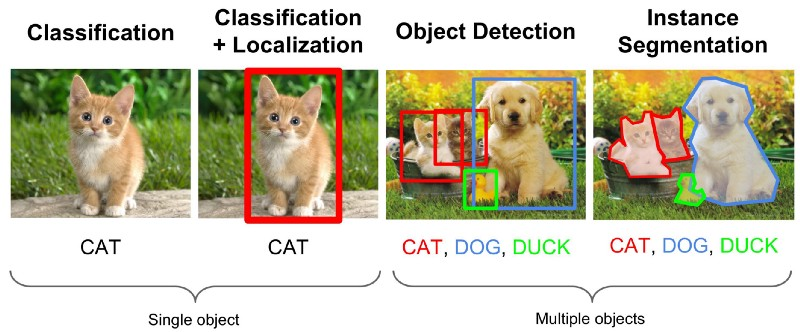
\includegraphics[width=0.9\textwidth]{figures/class_detect_segment.jpeg}
	\caption{Clasificare de imagine, localizare, detecție de obiecte, segmentare semantică \cite{class_detect_segment}}
	\label{fig:class_detect_semgent}
\end{figure}
\section{Domeniile din care face parte această lucare}
\subsection{Viziunea Artificială}
Viziunea artificială este un domeniu interdisciplinar care se ocupă cu metode cu ajutorul cărora calculatoarele pot să câstige o întelegere la un nivel ridicat și abstract ale imaginilor digitale. Scopul este automatizarea proceselor de care sistemul vizual human este capabil.\newline
Problemele în acest domeniu se pot încadra în mai multe categorii cum ar fi obținerea, procesarea, analiza și întelegerea imaginilor digitale. \textit{Înțelegerea} în acest context înseamnă transformarea imaginilor vizuale în descrieri, care la rândul lor pot fi folosite în alte procese (e.g. luarea deciziilor). După \cite{Szeliski10computervision} viziunea artificială este folosită în următoarele domenii:
\begin{itemize}
	\item controlul proceselor, inspecție automatică
	\item navigare
	\item probleme de clasificare și organizare
	\item detectare de evenimente
	\item recunoaștere de obiecte, identificare (e.g. persounei după amprentă sau față, etc.), detectare (e.g. verificarea prezenței unui obiect pe o imagine)
	\item analiza mișcărilor, reconstruirea scenelor, restorarea imaginilor, etc.
\end{itemize}
\subsubsection{Metode uzuale în domeniul viziunii artificiale}
În \cite{M82computervision} Kusuma Kumari B. M. face o prezentare generală a metodelor des folosite în domeniul viziunii artificiale și procesarea imaginilor.\newline
După ce am obținut o imagine digitală, urmează pasul de \textbf{pre-procesare}. În acest pas putem aplica operații de re-sampling, intensificarea sau micșorarea contrastului, operații pentru a reduce zgomotul din imagine, transformări de culoare (binarizare, grayscale, etc.).\newline
Odată ce imaginea atinge o calitate anume (și putem să avem încredere că algoritmii următori pot să prelucreze imaginea) urmează de obicei pasul de \textbf{extragerea trăsăturilor}. Imaginea este scanată pentru trăsături specifice (astea aflându-se la o granularitate mare sau mică) care împreună definesc un obiect complex. De obicei cautăm linii, muchii, colțuri, puncte, cercuri, creste, etc.\newline
Am ajuns la pasul în care folosind trăsăturile extrase la pasul anterior facem o \textbf{procesare} la nivel înalt. Deja trebuie să lucrăm numai cu trăsăturile extrase, aceasta fiind o mare îmbunătățire față de situația ipotetică în care ar trebui să lucrăm cu imaginea digitală de intrare. Pe baza trasăturilor extrase putem să executăm recunoașteri de obiecte, sau să aplicăm alți algoritmi pe multitudinea trăsăturilor (de exemplu pentru construirea unei imagini noi).\newline
În anumite cazuri mai este un pas, și anume \textbf{luarea deciziilor}. Aici pe baza tuturor pașilor anteriori programul ia o decizie, cu asta împlinind funcționalitatea completă.
\subsection{Rețele Neuronale}
În această secțiune o să fie prezentată ideea de bază a funcționării rețelelor neuronale cu ajutorul unor articole.\newline
Dorffner ș.a. în \cite{dorffner1996neural} prezintă funcționarea de bază a rețelelor neuronale; rețelele neuronale artificiale sunt inspirate de natură, acestea încercând să reproducă funcționarea rețelelor de neuroni din sistemul nervos al animalelor. O rețea neuronală artificială ca și cea "naturală" este construită din neuroni care alcătuiesc straturi de neuroni. Neuronii din două straturi consecutive sunt legate, legătura având o pondere: un număr care exprimă puterea legăturii dintre cei doi neuroni.\newline
În \cite{rojas1996backpropagation} Rojas ș.a. prezintă conceptul care stă la baza antrenării unei rețele neuronale: retropropagarea erorii. 	Acest algoritm pornește de la un \textit{set de date de antrenare} format din perechi intrare - ieșire dorită. Ponderele rețelei se inițializează cu valori aleatorii, alese de obicei din intervalul (-1, 1).\newline
Algoritmul (în cea mai simplă formă a ei) are două stagii:
\begin{enumerate}
	\item rețeaua neuronală primește o intrare din setul de antrenare. Folosind valorile curente ale ponderilor se face propagarea înainte a informației de intrare, calculându-se ieșirea reală furnizată de rețea
	\item ieșirea reală se compară cu valoarea dorită corespunzătoare setului de antrenare si eroarea calculată astfel se propagă înapoi în rețea - de la stratul de ieșire, spre stratul de intrare - pentru modificarea ponderilor.
\end{enumerate}
În \cite{aima} autorii specifică caracteristicile definitive a unei rețele neuronale artificiale, astea fiind:
\begin{itemize}
	\item architectura rețelei este definită de mai multe aspecte: numărul straturilor de neuroni, numărul neuronilor pe fiecare strat, ponderile rețelei, etc.
	\item regula de învățare (learning rule) este mechanismul responsabil pentru ajustarea ponderilor în iterațiile învățării. Alegerea aceste reguli poate diferenția între eșec și succes
	\item regula de activare a unui neuron: ce se întâmplă internal în fiecare neuron? Cum sunt intrările lui prelucrate pentru a obține ieșirea? Regula de activare este descrisă de funcția de activare.
\end{itemize}
\subsection{Rețele neuronale convoluționale}
Pal, Nikhil R and Pal și Sankar K în \cite{pal1993review} prezintă că dintre technicile de segmentarea imaginilor, rețelele neuronale convoluționale întrec celelalte abordări cu o margine semnificativă.\newline
Rețelele neuronale convoluționale sunt foarte similare cu rețelele neuronale profunde clasice: sunt alcătuite din neuroni care au ponderi pe care pot să le învețe. Fiecare neuron are intrări, aplică funcția de activare și propagă mai departe activarea produsă.\newline
Deci ce se schimbă? Architecturile convoluționale se bazează pe asumpția explicită, că intrările sunt \textbf{imagini}. Această asumpție ne împuternicesc să facem o architectură mai avantajoasă. Astfel pasul de propagare înainte devine mai eficientă iar costurile de antrenare se micșorează dat fiind faptul că numărul parametrilor se micșorează grozav.
În \cite{csfromuniversity} se prezintă de ce avem nevoie de îmbunătățirea oferită de rețelele convoluționale: rețelele neuronale regulare nu se scalează bine pentru imagini mari. În datase-ul CIFAR-10 imaginile au numai mărimea de 32x32x3 (32 lățime, 32 înălțime, 3 canale de culori), deci un strat complet conectat ar conține 32*32*3 = 3072 ponderi. Chiar dacă acest număr pare maniabil, se vede clar că structura fully-connected nu se scalează pentru imagini mari. De exemplu o poză color, cu o rezoluție de 200x200 pixeli ar avea nevoie de 200*200*3 = 120,000 ponderi.\newline
Rețelele convoluționale elimină problema numerelor mari prin punerea în practică a două idei: folosirea straturilor convoluționale și a straturilor de pooling. Dintre astea două straturile convoluționale fac marea parte a computărilor. Un strat convoluțional este alcătuit de fapt de în set de filtre; fiecare extrage trăsăturile corespunzătoare lui, și construieste o mapă de activări.\newline
Acum să vorbim despre detecția de obiecte și segmentarea semantică a unei imagini folosind rețele neuronale convoluționale...
\subsection{Detecția Obiectelor și Segmentarea Imaginilor Folosind Rețele Neuronale}
În \cite{historyCNN} Dhruv Parthasarathy prezintă că pentru detecția obiectelor și segmentarea semantică, cele mai bune rezultate sunt produse de rețele neuronale tip R-CNN (Regional Convolutional Neural Network). R-CNN are ca scop găsirea obiectelor principale în imagine (prin identificarea unui bounding box pentru fiecare) precum și clasificarea acestora într-o categorie. Intrarea în R-CNN este o imagine, iar ieșirea este un set de bounding boxes plus lista etichetelor obiectelor din imaginea de la intrare. Dar cum poate să specifice bounding box pentru obiecte? Ideea de bază a R-CNN este foarte intuitivă - se generează o miltitudine de regiuni în imagine și pentru fiecare se verifică cu ce probabilitate se poate clasifica obiectul din interior.\newline
%image showing how selective search proposes regions
\begin{figure}[h!]
    	\centering
	\captionsetup{justification=centering, margin=2cm}
	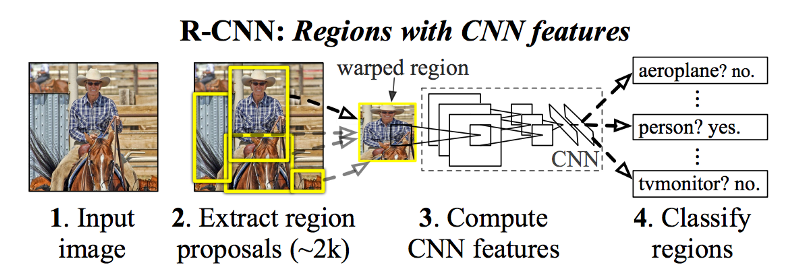
\includegraphics[width=0.9\textwidth]{figures/selective_search.png}
	\caption{Selective Search \cite{selective_search}}
	\label{fig:selective_search}
\end{figure}
Regiunile astea nu se generează la întâmplare, ci cu ajutorul unui algoritm: Selective Search. Selective search se uită pe imaginea completă, și generează regiunile astfel încât astea să conțină pixelii adiacenți care pot fi grupați împreună, cum ar fi: pixeli cu culoare asemănătoare, texturi asemănătoare, intensitate asemănătoare, etc.\newline

Odată ce regiunile (cu potențial mare de a conține un obiect) sunt generate de către selective search, R-CNN le clasifică cu o versiune modificată a rețelei AlexNet. Pe ultimul strat din rețeaua neuronală, se decide dacă regiunea încercată este într-adevăr un obiect, și dacă răspunsul este da, atunci ce fel de obiect?\newline
Cu toate că R-CNN funcționează coret, are un singur dezavantaj destul de serios, și anume: este foarte lent atât la folosirea propriu zisă cât și la faza de antrenare. Pentru toate ~2000 de regiuni generate cu selective search, se face o propagare înainte prin rețeaua neuronală (AlexNet), ceea ce înseamnă 2000 clasificări per imagine. Acest lucru nu se scalează bine și nu are șansa de a funcționa în timp real pentru captări video.\newline
În anul 2015, Ross Girshick (creatorul R-CNN) a rezolvat ambele probleme prin crearea unui nou algoritm numit Fast R-CNN. Să vedem care sunt ămbunătățirile aduse de acest sistem?
\begin{itemize}
	\item RoI Pooling (Region of Interest Pooling): s-a recunoscut faptul că când se efectuează pasul de propagare înainte pentru cele ~2000 regiuni propuse, sunt foarte multe suprapuneri. Îmbunătățirea constă în realizarea faptei, că în loc de a rula pe toate regiunile o clasificare, am putea să rulăm rețeaua neuronală o dată pe toată imaginea dacă găsim o metodă pentru împărtășirea acestei computatații pentru toate regiunile propuse (\ref{fig:roi_pooling}).
	\item Combinarea tuturor modelelor într-o rețea: în Fast R-CNN rețeaua neuronală convoluțională, clasificatorul și generatorul de regiuni sunt antrenate împreună. Unde în R-CNN am avut modele separate pentru extragerea trăsăturilor cu CNN, pentru clasificare (Support Vector Machine) și pentru generarea regiunilor de interest (Selective Search), acolo în Fast R-CNN se folosește o singură rețea pentru calcularea tuturor.
\end{itemize}
%image how RoI pooling works
\begin{figure}[h!]
    	\centering
	\captionsetup{justification=centering, margin=2cm}
	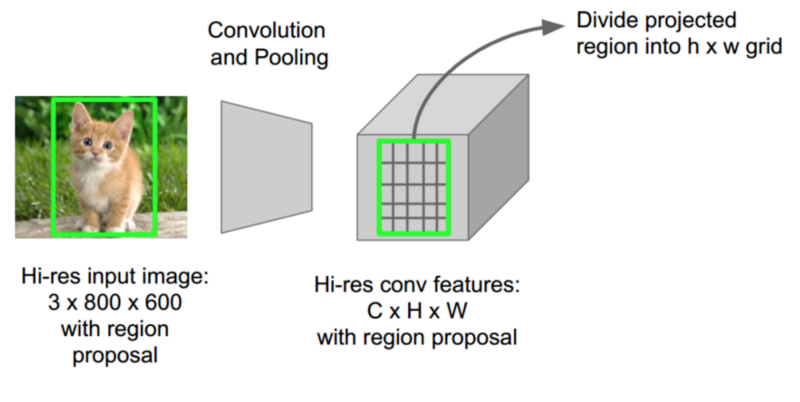
\includegraphics[width=0.7\textwidth]{figures/fast_rcnn.png}
	\caption{RoI Pooling \cite{historyCNN}}
	\label{fig:roi_pooling}
\end{figure}




%image showing that neural networks outperform humans on the ILSVRC
\begin{figure}[h!]
    	\centering
	\captionsetup{justification=centering, margin=2cm}
	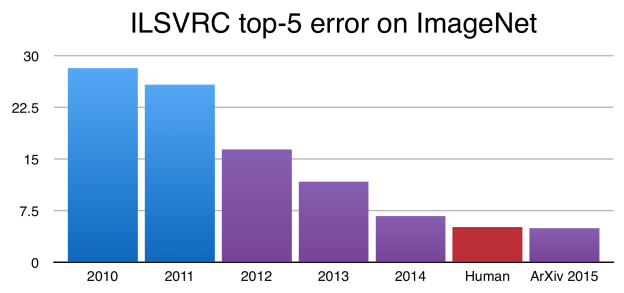
\includegraphics[width=0.9\textwidth]{figures/top_five_errors_ILSVRC.png}
	\caption{Rețelele neuronale convoluționale obțin punctaj mai mare decât oamenii în clasificarea obiectelor \cite{historyCNN}}
	\label{fig:historyCNN}
\end{figure}


Documentarea bibliografică are ca obiectiv fixarea referențialului în care se situează tema, prezentarea susrselor bibliografice utilizate și a cercetărilor similare și raportarea abordării din lucrare la acestea.

Referințele bibliografice se vor face pentru fiecare carte, articol sau material folosit pentru elaborarea lucrării de licență. 

Reprezintă cca. 10--15\% din lucrare.


% \section{Related Work}
\section{Abordări similare}

Comparați abordarea voastră cu cele ale altor soluții: ce e asemănător, ce e diferit (și, de preferat, mai bun). 

Citarea referințelor se face ca în exemplele \ref{subsec:s10} din Bibliografie. 
Vezi citările următoare.

În articolul \cite{Antoniou04} autorul descrie configurația tehnică a unei "honeynet" și prezintă câteva atacuri de actualitate asupra honeynet, precum și o serie de recomandări pentru securizarea sistemelor conectate la rețele de calculatoare.

% În capitolul 4 al [], referitor la valoare honeypots, Spitzner prezintă avantajele și dezavantajele acestora.

În articolul on-line \cite{electronic-citation} găsim detalii interesante despre \dots.


% \section{Technologies and Methods}
\section{Tehnici/Tehnologii/Surse folosite}

Sursele de documentare referitoare la metodele, tehnologiile, ideile folosite. 




% \chapter{Theoretical Backgound}
\chapter{Fundamente teoretice}
În acest capitol se vor prezenta fundamentele teoretice proiectului, și se vor explica în detaliu deciziile architecturale luate în elaborarea proiectului.\newline
Scopul proiectului a fost proiectarea și implementarea unui program/sistem care este capabil să clasifice obiecte din imagini, să poată face detecția obictelor (adică să specifice unde se află acestea în imagine) și să facă segmentarea semantică a imaginii. Am ajuns la decizia că pentru aceste probleme o să folosesc o rețea neuronală convoluțională deoarece rețelele neuronale depășesc orice altă abordare capabilă să efectueze aceste sarcini.\newline
În primul rând o să se facă prezentarea rețelelor neuronale (convoluționale) și straturile specifice acestora. După aceasta vom afla cum se întâmplă antrenarea rețelei.




\section{Rețele Neuronale Convoluționale}
O rețea neuronală convoluțională - ca orice rețea neuronală - are la bază conceptul de \textit{neuron}, acesta fiind elementul din care se construiește. Aceștia sunt organizați în \textit{straturi de neuroni} (layer), straturile fiind interconectate formând o \textit{ierarhie de straturi}.\newline
Informația de intrare este alimentată \textit{stratului de intrare} (input layer). După aceasta semnaul se propagă printr-o serie de \textit{straturi ascunse}; în fiecare strat neuronii își calculează activarea prin folosirea \textit{funcției de activare}, iar activările se propagă în direcția \textit{stratului de ieșire} (output layer). Stratul de ieșire la rândul lui va furniza informația necesară (e.g. clasificarea obiectului din imagine, detecția obiectelor, segmentarea semantică, etc.).




\subsection{Neuronul Artificial}
În contextul științei biologiei neuronul este o celulă, un bloc de construcție, a cărui rol este colectarea semnalelor de la neuronii vecini prin dentriți, procesarea acestor informații, și pe baza informațiilor obținute și a structurii interne emite un semnal al lui prin axonul lui.\newline
%image of biological neuron
\begin{figure}[h!]
    	\centering
	\captionsetup{justification=centering, margin=2cm}
	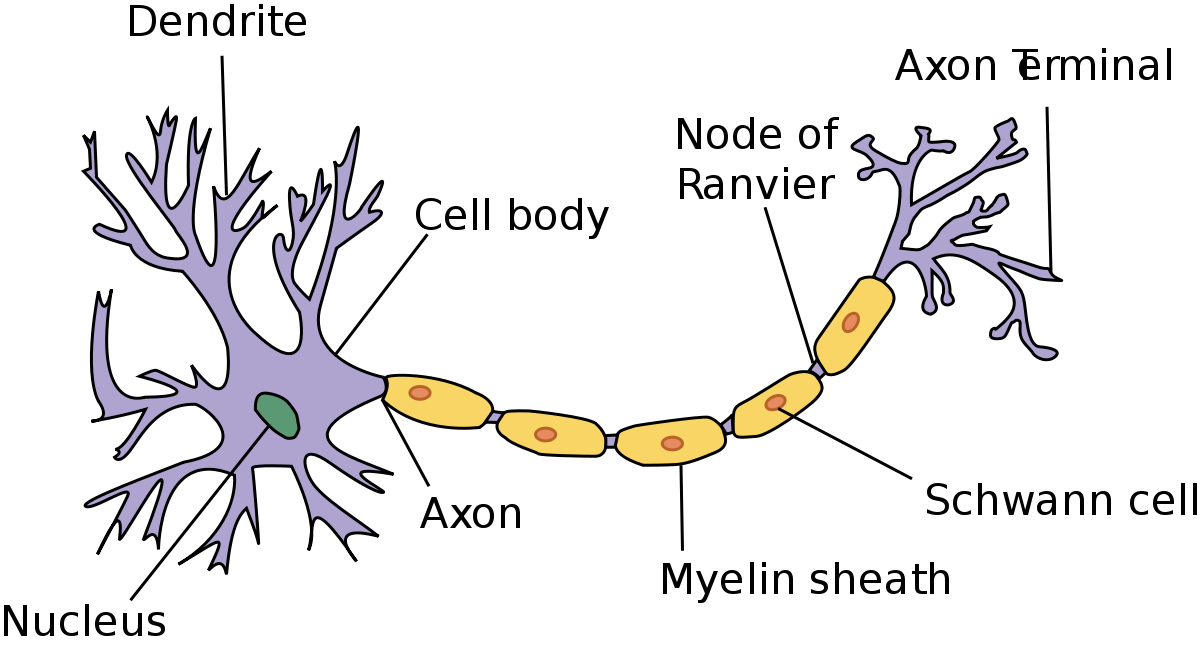
\includegraphics[width=0.5\textwidth]{figures/neuron.png}
	\caption{Neuronul - blocul de construcție a sistemului nervos \cite{neuron}}
	\label{fig:segmentare_semantica}
\end{figure}
Ideea neuronului artificial este bazată pe aceeași idee, părțile din care se compune fiind:
\begin{itemize}
	\item Intrările ponderate: semnalele/activările stratului anterior în șir sunt ponderate, asta însemnând că un neuron poate fi mai mult sau mai puțin influențat de un alt neuron. Ponderile sunt învățate în faza antrenării rețelei. Prin ponderi se introduce conceptul de \textit{neurons that fire together wire together}.
	\item Funcție de activare: pe baza intrărilor se calculează cât de tare este activat acest neuron.
	\item Ieșire: semnalul de activare se propagă la neuronii din stratul următor prin ieșirea lui.
\end{itemize}
%image of biological neuron
\begin{figure}[h!]
    	\centering
	\captionsetup{justification=centering, margin=2cm}
	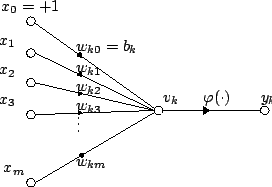
\includegraphics[width=0.5\textwidth]{figures/an.png}
	\caption{Modelul neuronului artificial \cite{arn}}
	\label{fig:neuronul_artificial}
\end{figure}

Neuronul biologic se activează (dă un semnal de ieșire) numai dacă semnalul de intrare depășește un anumit prag. În rețelele neuronale artificiale acest efect este simulat aplicând \textit{sumei ponderate} a intrărilor o fincție de transfer (activare) pentru a obține semnalul de ieșire.



\subsubsection{Descrierea matematică a funcționării unui neuron}
Întrările unui neuron se pot percepe ca o matrice de numere (fiecare fiind activarea unui neuron de pe stratul anterior) având $R$ elemente. Intrările individuale $p_1, p_2, \dots, p_R$ sunt înmulțite cu ponderile $w_{1,1}, w_{1,2}, \dots, w_{1,R},$ și valorile ponderate se însumează. Suma se poate nota cu \textbf{Wp}, adică produsul scalar al matricei \textbf{W} și vectorul \textbf{p}.\newline
Neuronul are \textit{ b (bias)}, care se adună cu intrările ponderate, rezultând arguentul $n$ al funcției de transfer
\begin{equation}
f: w_{1,1}p_1 + w_{1,2}p_2 + \dots + w_{1,R}p_R + b = n
\end{equation}
Această poate fi scrisă cu notația abreviată:
\begin{equation}
n = W*p + b; a = f(n)
\end{equation}


% enumerate the usual activation functions of neurons
Dacă ne uităm la funcțiile de transfer a neuronilor artificiali des folosite, vedem că există mai multe tipuri sau categorii de neuroni acestea fiind:
\begin{itemize}
	\item \textit{Threshlod neurons} (neuronii cu funcția treaptă): acest tip de neuron are cea mai simplă funcție de activare; ia intrările de la neuronii din stratul anterior, multiplică activările acestora cu ponderea respectivă pentru fiecare și calculează suma numerelor obținute după înmulțire. Înainte de a da ai departe rezultatul, se mai scade un număr special, numit \textit{bias}. Dacă rezultatul scăderii este mai mare decât zero, atunci ieșirea neuronului este unu, altfel zero.
\begin{equation}
	activation =
		\begin{cases}
			1, \text{if } n > 0 \\
			0, \text{otherwise}
		\end{cases}
\end{equation}
	\item \textit{Linear combination neuron} (neuronii cu funcția de transfer liniară - purelin): acest tip de neuron se comportă asemănător cu neuronii de prag. Ia intrările, calculează suma intrărilor ponderate și din această sumă scade bias-ul. Dacă rezultatul este mai mic decât zero, atunci activarea acestui neuron va fi zero. Între zero și unu, se propagă mai departe valoarea calculată. Peste unu, valoarea trimisă mai departe va fi și ea unu.
\begin{equation}
	activation = purelin(n)
\end{equation}
	\item \textit{Sigmoid neuron}:  neuronii care fac parte din această categorie folosessc o funcție non-liniară pentru a calcula activările lor: funcția sigmoidală. Această funcție este aleasă fiindcă calcularea derivativei ei este ușoară aceasta fiind a caracteristică crucială pentru a face posibilă antrenarea rețelei cu ajutorul algoritmului \textit{baskpropagation}.
\begin{equation}
	a = \frac{1}{1 + \mathrm{e}^{-n}}
\end{equation}
\end{itemize}

%image of biological neuron
\begin{figure}[h!]
    	\centering
	\captionsetup{justification=centering, margin=2cm}
	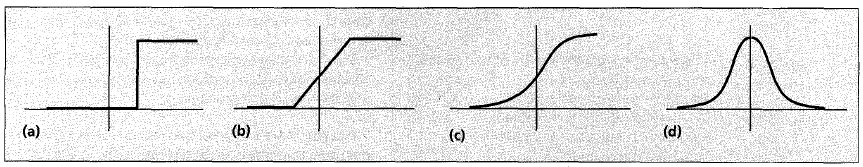
\includegraphics[width=0.7\textwidth]{figures/activation_functions.png}
	\caption{Funcții de transfer \cite{activationFunctions}}
	\label{fig:activationFunctions}
\end{figure}



\subsection{Rețeaua Neuronală Artificială}
Acum că am stabilit ce este un neuron artificial, categoriile neuronilor și funcționarea fiecăruia, putem lua un pas înapoi să vedem imaginea întreagă: rețeaua neuronală artificială care este construită din neuroni.\newline
Rețelele neuronale artificiale sunt utilizate pe scală largă în contextul inteligenței artificiale. Modelul și modul de funcționare a acestora este inspirată de modelul rețelelor neuronale din sistemul nervos al animalelor și al omului (imitând funcționarea sistemului nervos central sau a creierului).\newline
Popularitatea lor provine din faptul că acestea sunt capabile de a învăța funcți incredibil de complexe, cu mii de parametri (datoritp numărului mare de ponderi care pot fi învățate pentru a ajunge la o estimare cu ajustare precisă). Rețelel neuronale au urmâtoarele caracteristici importante:
\begin{itemize}
	\item Architectură: aceasta cuprinde decizii asupra numărului de straturi de neuroni, parametrii ca și numărul neuronilor pe fiecare strat aparte, ponderile conexiunilor, și inițializarea acestora.
	\item Regula de învățare/algoritmul de învățare: este mechanismul ales care va îndeplini sarcina ajustării ponderilor în fiecare iterație de antrenare. Alegerea algoritmului corespunzător este de o importanță crucială, și trebuie examinată pentru că un algoritm necorespunzător ar putea rezulta în incapabiliatea de a antrena rețeaua.
	\item Funcțiile de transfer a neuronilor din fiecare strat
\end{itemize}

% NeuNet with one hidden layer IMAGE
\begin{figure}[h!]
    	\centering
	\captionsetup{justification=centering, margin=2cm}
	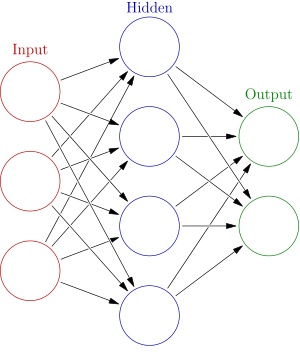
\includegraphics[width=0.3\textwidth]{figures/artificialneunet_1hidden.png}
	\caption{O rețea neuronală artificială cu un singur strat ascuns \cite{arn}}
	\label{fig:activationFunctions}
\end{figure}
Rețelele neuronale au o serie de straturi de neuroni, acestea de obicei fiind numerotate de la $L_0$ până la $L_N-1$ unde N este adâncimea rețelei neuronale. Neuronii de pe stratul $L_i$ primesc intrările de la stratul anterior, $L_i-1$. Folosind aceste intrări neuronul aplică funcția lui de transfer, rezultatul fiin activarea neuronului. Această activare se propagă mai departe spre stratul următor, adică $L_i+1$ unde va constitui parte din intrările neuronilor.


Între două straturi de neuroni vecini există $R*S$ ponderi, $R$ și $S$ fiind numărul neuronilor pe cele două straturi. De reguă aceste ponderi sunt organizate într-o matrice de ponderi:
\begin{equation}
	W = \begin{bmatrix}
		w_{1,1} && w_{1,2} && \dots && w_{1,R} \\
		w_{2,1} && w_{2,2} && \dots && w_{2,R} \\
		\dots && \dots && \dots && \dots\\
		w_{S,1} && w_{S,2} && \dots && w_{S, R} \\
	\end{bmatrix}
\end{equation}



\subsubsection{Rețele neuronale cu straturi multiple de neuroni}
O rețea neuronală artificială poate acea mai multe straturi, fiecare strat având o matrice a ponderilor \textbf{W}, un vector al deplasărilor \textbf{b} și un vector de ieșire \textbf{a}. Pentru a distinge matricile ponderilor, vectorii de ieșire, etc., pentru fiecare strat din rețea notăm numărul stratului ca superscript la variabila respectivă. O intrare constantă este atașată fiecărui neuron, asta fiindu-i \textit{deplasarea (bias)}. Ieșirile din fiecare strat intermediar reprezintă intrările pentru stratul următor. Astfel, stratul $i$ are $S^{i-1}$ intrări, $S^{i}$ neuroni și o matrice $W^2$ a ponderilor (cu dimensiunile $S^{i}\times S^{i-1}$). Intrarea in stratul $S^{i}$ este $a^{i-1}$, iar ieșirea este $a^{i}$. Această abordare se poate aplica oricărui strat din rețea.\newline
Straturile pot avea roluri diferite:
\begin{itemize}
	\item stratul care produce ieșirea rețelei este numit \textit{strat de ieșire}
	\item celelalte straturi se numesc \textit{straturi ascunse}
\end{itemize}
Ieșirea ultimului strat este ieșirea rețelei, și se notează cu $y$. Rețelele multi-strat sunt foarte eficiente. De obicei acestea au mai multe straturi ascunse cu neuroni sigmoidali, urmate de un strat de neuroni liniari. Fiindcă există mai multe straturi de neuroni cu funcție non-liniară de transfer, rețeaua este capabilă să învețe atât funcții liniare cât și funcții neliniare. Ultimul strat liniar permite rețelei să producă și rezultate care sunt în afara intervalului $[-1, 1]$.


\subsection{Antrenarea}
În această secțiune se va prezenta conceptul de \textit{machine learning} în contextul inteligenței artificiale, și cum învață rețelele neuronale (prin explicarea funcționării algoritmului de propagare inversă a erorii).\newline

\subsubsection{Machine Learning}
Este un domeniu a științei calculatoarelor care se ocupă cu algoritmi care cunt capabili de a generaliza, a învăța concepte care nu erau programate explicit. În această lucrare se folosesc rețele neuronale artificiale pentru a învăța concepte complexe precum recunoașterea obiectelor din imagini (mai particular se va vorbi despre învățarea supravegheată).

\paragraph{Metodele de învățare}


\subparagraph{Învățarea Supravegheată} \textit{(supervised learning)} presupune în orice moment (pentru orice set de date de intrare) existența unei valori dorite ($target$) pentru fiecare neuron din stratul de ieșire a rețelei. Sistemului i se furnizează seturi de perechi de intrare-ieșire dorită cu ajutorul cărora se calculează mrimi de eroare în funcție de diferența dintre valoarea reală a ieșirii și cea dorită, pe baza cărora se ajustează valorile parametrilor rețelei (interconexiuni și eventual valori de prag ale funcțiilor de activare). 


\subparagraph{Învățarea Nesupravegheată} \textit{(unsupervised learning)} rețeaua extrage singură anumite caracteristici importante a datelor de intrare formând reprezentări interne distincte ale acestora. Rețeaua nu beneficiază de seturi de ieșire dorite, în schimb se utilizează un gen de "competiție" între neuronii elementari care are ca efect modificarea conexiunilor aferente numai neuronului care "câștigă" întrecerea, restul legăturilor rămânând neafectate.


\subparagraph{Învățarea folosing un "critic"} \textit{(reinforcement learning)} este denumită uneori și cu recompensă/pedeapsă ($reward/punishment$). În această situație, rețeaua nu beneficiază de un semnal dorit ca în cazul învățării supravegheate, ci de un semnal care oferă o informație calitativă ilustrând cât de bine funcționează sistemul (informația este binară, de tipul "răspunsul este bun/greșit"). Algoritmii aparținând acestei categorii sunt inspirați într-o mai mare măsură de observații experimentale făcute pe animale și, în esență, funcționează după următorul principiu: dacă urmarea unei anumite acțiuni întreprinse de un sistem capabil să învețe are un efect favorabil, tendința de a produce acțiunea respectivă în situația respectivă este încurajată, în caz contrar este inhibitată.


\subsection{Antrenarea Rețelelor Neuronale}
După ce ponderile și deplasările rețelei au fost inițializate, rețeaua este pregătită pentru a fi antrenată. Procesul de antrenare necesită un set mare de valori privind comportarea rețelei: intrări in rețea $p$ și ținta ($target$) t. În timpul antrenării, ponderile și deplasările sunt ajustate iterativ pentru ca rețeaua neuronală să greșească cât mai puțin.\newline


\subsubsection{Funcția de cost} Funcția de cost este funcția folosită pentru specificarea erorii pe care a făcut rețeaua pentru un set dat de intrări-ieșiri dorite. Pentru fiecare stare a rețelei neuronale putem asigna o valoare numerică, cu care putem descrie eroarea. Această valoare se numește \textit{cost}.\newline
Cu cât costul este mai mare, cu atât rețeaua este mai departe de starea în care am dori să fie. Cum se micșoreză costul, așa rețeaua neuronală ajunge mai aproape de o configurație a parametrilor în care produce predicțiile pe care le-am dori. Valoarea costului este calculată de \textit{funcția de cost}. Zicem că un model este $optimal$ dacă nu putem găsi o altă asignare a valorilor parametrilor rețelei astfel încât să ne producă un cost mai mic.\newline
Cu toate aceste noțiuni explicate, putem formula ce ar însemna învățarea/antrenarea pentru rețele neuronale: antrenarea este procesul iterativ prin care în fieare iterație costul rețelei neuronale scade, asta însemnând că pas cu pas predicțiile rețelei ajung mai aproape de realitate. În fiecare iterație de antrenare vrem să modificăm valorile ponderilor interconexiunilor și valorilor deplasărilor astfel încât să scadă costul. Pentru a atinge acest scop, de regulă se folosește algoritmul numit $propagarea inversă a erorii$.


\subsubsection{Propagare Inversă și Metoda Gradientului Negativ}
Cea mai simplă interpretare a algoritmului de propagare inversă actualizează ponderile rețelei și deplasările în direcția în care funcția de performanță scade cel mai rapid, adică în direcția gradientului negativ.\newline
Dacă am avea o singură pondere într-o rețea, atunci optimizarea rețelei ar fi destul de simplă: am putea încerca toate valorile pentru ponderea respectivă și am putea alege valoarea cu care primim cel mai bun rezultat. Problema este că dacă numărul de ponderi este mai mare, atunci această abordare devine incredibil de ineficientă. Aici vine ideea vicleană a propagării inverse: nu suntem nevoiți să încercăm toate configurațiile de ponderi și deplasări; de fapt ajunge să le inițializăm la întâmplare, și după aceasta le actualizăm iterativ astfel încât în fiecare iterație să ajungem la un cost mai mic decât în iterația anterioară astfel ajungând la o soluție mai aproape de cea optimă.\newline


\paragraph{Descrierea matematică a metodei gradientului negativ}
Să fie $F(x)$ o funcție multi-variabilă, care se poate deriva în vecinătatea punctului $a$. Atunci, dacă vrem să aflăm setul variabilelor care care conduc spre minimul funcției, ar trebui să luăm un $pas$ din $a$ în direcția speficicată de gradientul negativ a funcției $F$ în punctul $a$:
\begin{equation}
	b = a - \gamma \nabla F(a).
\end{equation}
Acesta va asigura, că $F(b) < F(a)$ însemnând ca punctul $b$ este mai aproape de minimul funcției $F$.


%visualization of gradient descent
\begin{figure}[h!]
    	\centering
	\captionsetup{justification=centering, margin=2cm}
	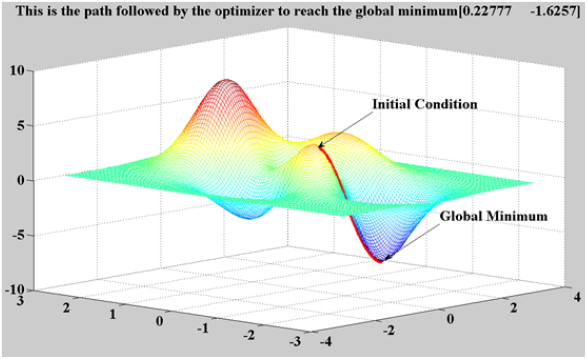
\includegraphics[width=0.9\textwidth]{figures/gradient_descent.png}
	\caption{Vizualizarea metodei gradientului negativ pentru o funcție cu două variabile \cite{arn}}
	\label{fig:gradient_descent}
\end{figure}

Repetând acest proces (calcularea gradientului în punctul curent, și actualizarea parametrilor prin scăderea gradientului), dacă pasul de învățare este destul de mic, atunci vom converga către un minim local. Dacă funcția $F$ este una convexă, atunci metoda gradientului invers ca converga către un punct foarte apropiat de minimul global.

\paragraph{Propagarea inversă}
Metoda propagării inverse a erorii este aplicată pe scală largă în domeniul rețelelor neuronale, la procesul de antrenare. Este folosit împreună cu metode de optimizare cum ar fi metoda gradientului negativ.\newline
Metoda constă din calcularea gradientului funcției de cost $C$, pentru fiecare pondere a rețelei neuronale. După ce gradientul funcției de cost este calculat, acesta este dat metodei de optimizare (gradient negativ), care pe baza gradientului actualizează ponderile interconexiunilor dintre neuroni și deplasările acestora. Astfel în fiecare iterație de antrenare, valoarea erorii este propagată dinspre stratul de ieșire către stratul de intrare, actualizând întreaga rețea.\newline
Această metodă de antrenare necesită un set de antrenare care conține atât exemple cât și predicția dorită pentru fiecare, pentru că folosind predicțiile dorite putem să calculăm eroarea (sau costul) rețelei pentru un set de intrări. Când antrenăm o rețea neuronală folosing propagarea inversă, evenimentele se pot separa în două faze:\newline

\subparagraph{Propagarea Înainte și Propagare Inversă} constituie propagarea activărilor neuronilor dinspre stratul de intrare către stratul de ieșire și propagarea inversă a erorii calculate de la stratul de ieșire spre stratul de intrare. Când semnalul ajunge la stratul de ieșire, se calculează diferența dintre predicția rețelei neuronale și \textit{target}-ul dorit. Pasul doi este propagarea acestei erori înapot, pentru a afla cum trebuie actualizate ponderile interconexiunilor și deplasările neuronilor.

\subparagraph{Weight Update} este faza în care se aplică următorii pași: înmulțim diferența fiecăruii nod cu semnalele de intrare; așa primim gradientul cu privire la ponderea conexiunii. În al doilea pas scădem o parte a gradientului punctului respectiv din ponderile nodului.\newline
\begin{equation}
	W \prime = W-\alpha \nabla ,
\end{equation}
unde $\alpha$ este rata de învățare (\textit{learning rate/learning speed}). Valoarea lui $\alpha$ se poate schimba dinamic între iterații de învățare, dar rămâne constant în timpul unei iterații. Valoarea și algoritmul de actualizare a ei trebuie aleasă cu mare grijă. Un $\alpha$ mai mare este echivalent cu luarea unor pași mai mari în jos, spre minimul funcției de cost/performanță. Acest lucru este dorit fiindcă rețeaua învață mai repede, dar are un dezavantaj foarte important: dacă pasul de învățare este una prea mare, atunci se poate întâmpla că pășim peste minimul suprafeței funcției de cost adică pășim peste soluția optimă fără să observăm. Pe de altă parte un $\alpha$ mai mic ne permite a să convergăm cu o acuratețe mai mare de soluția optimă, dar dezavantajul este că se poate bloca la fiecare minim local, nefiind capabil să iasă din punctele aparent bune (se poate opri la un punct foarte ne-optim pe suprafața de cost doar pentru că aceasta este un minim local.

\subsection{Date de Antrenare și Testare}
Antrenarea este faza în care rețeaua neuronală învață prin actualizarea ponderilor conexiunilor și actualizarea deplasărilor fiecărui neuron. Pentru a realiza antrenarea rețelei neuronale avem nevoie de un set de antrenare suficient de mare alcătuit din imagini etichetate (invățare supravegheată). Rețeaua neuronală face o predicție pe baza unei imagini din setul de antrenare, predicția fiindu-ne vizibilă la stratul de ieșire. Când eticheta ghicită de rețea apare la ieșire, calculăm un cost: diferența dintre predicția rețelei și valoarea adevărată, adică eticheta imaginei corespunzătoare. Având costul calculat suntem capabili să actualizăm ponderile și deplasările, astfel încât să-l micșorăm, folosing algoritmii prezentați mai sus. După o perioadă de antrenare (e.g. 1000 iterații de antrenare) avem o rețea neuronală a cărui ponderi sunt mai aproape de cele optimale decât parametrii rețelei nou-inițializate.\newline
Acum urmează pasul în care testăm cât de bine funcționează rețeaua neuronală. Avem la îndemână un set mare de imagini etichetate, care n-au fost folosite la antrenare. Comparăm predicțiile rețelei cu etichetele reale ale imaginilor și facem statistici privitoare la precizia predițiilor.


\section{Rețele Neuronale Convoluționale}
Rețelele neuronale convoluționale sunt un tip special a rețelelor neuronale, și s-au demonstrat foarte folositoare pentru recunoașterea, detecția și segmentarea imaginilor iar pentru analizarea semnalelor audio.\newline
Ele folosesc tipuri de straturi specifice rețelelor convoluționale.

\subsection{Straturi convoluționale}
Straturile convoluționale sunt alcătuite dintr-un set de filtre convoluționale (\textit{convolutional kernerls)}. După antrenarea rețelei astea devin niște filtre \textit{Gabor-like}.

%Gabor-like filters
\begin{figure}[h!]
    	\centering
	\captionsetup{justification=centering, margin=2cm}
	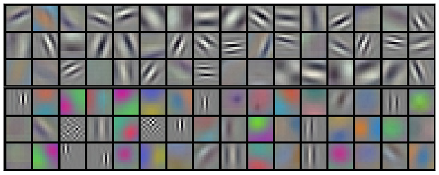
\includegraphics[width=0.9\textwidth]{figures/gabor_filters.png}
	\caption{set of Gabor filters \cite{gabor_filters}}
	\label{fig:set of Gabor filters}
\end{figure}

Straturile convoluționale au doi parametri pe care le putem modifica pentru a obține modificarea comportamentului fiecărui strat. După ce am ales dimensiunile stratului, trebuie să alegem \textit{stride} și \textit{padding}. \newline
Stride controlează cum filtrul convoluțional se mișcă pe suprafața matricii de pixeli a imaginii de intrare. \newline
De exemplu dacă $stride=1$ atunci filtrul este mișcat du pași de un pixel. De obicei valoarea parametrului stride se alege astfel încât imaginea generată de filtrul convoluțional să aibă dimensiuni de numere întregi nu fracții. Să luăm un exemplu: să ne imaginăm o imagine de intrare a carei dimensiune este 7x7 pixeli, și un filtru convoluțional de dimensiunea 3x3 cu un stride de un pixel.

%convolutional layer stride illustration
\begin{figure}[h!]
    	\centering
	\captionsetup{justification=centering, margin=2cm}
	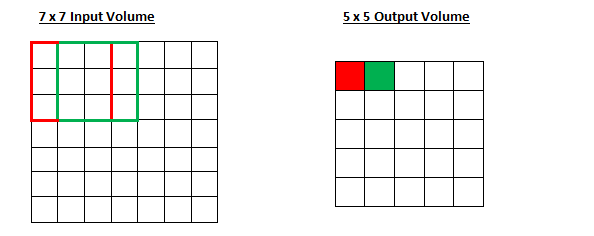
\includegraphics[width=0.9\textwidth]{figures/con_lay_stride.png}
	\caption{set of Gabor filters \cite{conv_lay_params}}
	\label{fig:con_lay_str}
\end{figure}


Pe figura\ref{fig:con_lay_str} putem vedea că matricea rezultată a valorilor produse de stratul convoluțional are dimensiunea de 5x5. Dar ce s-ar întâmpla dacă am folosi un stride de 2 pixeli? În acest caz pe axa orizontală putem să plasăm filtrul în trei poziții, la fel și pe axa verticală. Deci dimensiunile ieșirii filtrului are fi 3x3.\newline
Putem vedea că cu un stride mai mare ieșirea filtrului se micșorează. Putem observa și faptul că dacă stride ar fi trei, atunci am avea probleme cu plasarea filtrului. De obicei valoarea lui stride este mai mare decât unu dacă vrem ca regiunile receptive să nu se suprapună.\newline
Să aruncăm o privire și pe parametrul numit \textit{padding}. Înainte de a intra în detalii despre acest parameru, să cedem o situație reală: ce s-ar întâmpla dacă am aplica un filtru de 5x5 pe o imagine de 32x32? Dimensiunile ieșirii ar fi 28x28, deci imaginea se micșorează. Aplicând mai multe filtre convoluționale consecutive pe o imagine, ne lovim de o problemă: dimensiunile imaginii se reduc mai repede decât am dori. În primele straturi a rețelei neuronale dorim să conservăm cât mai multă informație.\newline
Să zicem că vrem să aplicăm același filtru convoluțional pe același imagine, dar de data asta ne folosim și de un padding, și anume: \textit{zero-padding}. Acesta înseamnă că mărim imaginea originală cu 2 pixeli in fiecare dimensiune, astfel ajungând la dimensiunea de 36x36. Elementelor nou-introduse în matrice le asignăm valoarea de 0.\newline
Ce am realizat cu introducerea paddingului este că după aplicarea aceluiași filtru (dimensiunea de 5x5 pixeli cu stride=1) imaginea rezultată nu mai este micșorată, ci rezultatul tot o să fie de 32x32.\newline
Formula pentru a calcula dimensiunile ieșirii pentru un strat convoluțional este
\begin{equation}
	O = \frac{W-K+2P}{S}+1
\end{equation}
unde K este dimensiunea filtrului, W este dimensiunea imaginii de intrare, P este valoarea paddingului și S este stride.


\subsection{Straturi nonlineare (Nonlinearity Layers)}
Aceste straturi acționează ca filtre nonlineare: intrarea este o matrice sau o imagine, peste care se aplică o activare \textit{non-saturating}. Pot fi de mai multe feluri:
\begin{itemize}
	\item ReLU: această funcție ia intrarea după ce aplică funcția de activare $f(x)=max(0, x)$. După ce a aplicat funcția de tranziție, propagă matricea sau imaginea rezultată mai departe,
	\item Tanh: această funcție ia intrarea și aplică funcția re activare $f(x)=tanh(x)$, după ce rezultatul este propagat mai departe,
	\item Sigmoid: acest tip de funcție ia intrarea peste care aplică funcția de tranziție $f(x)=exp(-x)+1$.
\end{itemize}

%non-linear activation functions
\begin{figure}[h!]
    	\centering
	\captionsetup{justification=centering, margin=2cm}
	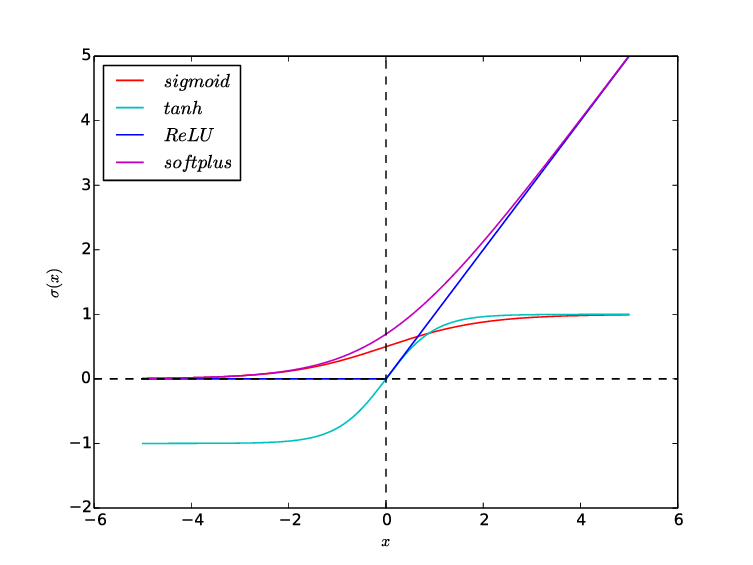
\includegraphics[width=0.9\textwidth]{figures/nonlinear_activation_functions.png}
	\caption{Funcțiile de transfer nonlineare \cite{non_lin_act_fun}}
	\label{fig:set of Gabor filters}
\end{figure}

\subsection{Local-Response Normalization Layers}
Acest tip de strat are ca intrare ieșirea de la stratul anterior și se folosește atunci când valorile de intrare pot fi infinit de mari. Acest strat normalizează într-un mod uniform intrările mari dintr-o regiune. Astfel face posibil ca activările foarte puternice să competizeze în grupuri de neuroni.

\subsection{Pooling Layers}
Acest tip de strat este specific rețelelor neuronale convoluționale; impune un \textit{downsampling} nonlinear a ieșirilor din stratul precedent. Există mai multe tipuri, cum ar fi max-pooling, average pooling, L2-norm pooling.\newline
Max-pooling este metoda cea mai des folosită, și funcționează în următorul fel: ca intrare se primeste o matrice sau o imagine. Această matrice sau imagine este partiționată în regiuni care nu se suprapun, regiunile având mărime bine definită. Din fiecare regiune se propagă mai departe numai cea mai puternică activare/cel mai puternic semnal. Acest fenomen are semnificația următoare: dacă într-o regiune am găsit a trăsătură fominantă, atunci poziția exactă a trăsăturii nu contează; este important numai să știm poziția relativă a acestei trăsături față de celelalte trăsături dominante.\newline
Beneficiul acestui tip de strat este acea că se reduce mărimea imaginii, extragându-se numai trăsăturile cele mai importante din ea. Ca urmare, după un strat pooling, numărul parametrilor rețelei se micșorează seminficativ fiindcă cantitatea informației din imagine se micșorează și ea. Astfel numărul ponderilor este redus drastic (75\%) reducând timpul și efortul de computație. Un alt beneficiu introdus de acest tip de strat este să controlează și \textbf{overfitting}ul. Overfitting este fenomenul prin care un model (o rețea neuronală) nu face generalizările necesare despre entitățile pe care trebuie să le recunoască, ci extrage și învațâ trăsături specifice din exemplele de antrenare. Principala simptomă a unei rețele care face overfitting este că pe setul de antrenare are o eficiență de peste 90\% dar numai 50\% pe setul de imagini de testare.

%max-pooling layer
\begin{figure}[h!]
    	\centering
	\captionsetup{justification=centering, margin=2cm}
	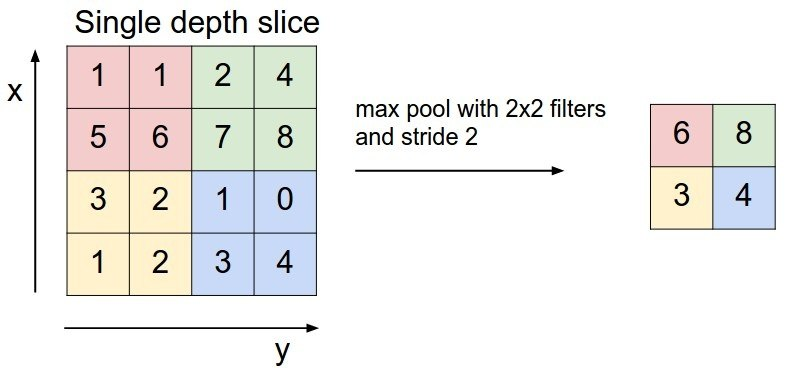
\includegraphics[width=0.9\textwidth]{figures/max_pol.jpg}
	\caption{Stratul max-pooling \cite{max_pol}}
	\label{fig:Stratul max-pooling }
\end{figure}

\subsection{Fully-Connected Layers}
Într-o rețea neuronală convoluțională, acest tip de strat execută sarcina predicției la nivel înalt. Se numește fully-connected pentru că neuronii din acest strat sunt interconectați cu fiecare neuron de pe stratul precedent.\newline
Activările stratului fully-connected pot fi calculate cu o simplă înmulțire între matrici (intre matricea de intrări și matricea de ponderi) și aplicând matricea de deplasare.

\subsection{Dropout Layer}
Acest tip de strat este prezent în rețelele neuronale convoluționale pentru a previne fenomenul de \textit{overfitting}. După antrenarea rețelei neuronale cu ajutorul setului de antrenare, scopul nostru este atingerea unei performanțe cât mai înalte pe setul de testare. Pentru a evita \textit{overfitting} și a induce un nivel mai mare de generalizare, straturile dropout fac următorul: iau neuroni cu probabilitate de $p=0.5$, pentru a fi scoase temporal din rețea. Muchiile de intrare și ieșire sunt scoase până la sfârșitul iterației.\newline
Astfel rețeaua neuronală are mai puține parametri în fiecare iterație, forțându-l să generalizeze în loc de overfitting. La sfârșitul fiecărei iterații neuronii eliminați sunt reintroduși în rețea cu ponderile neschimbate.

%dropout layer
\begin{figure}[h!]
    	\centering
	\captionsetup{justification=centering, margin=2cm}
	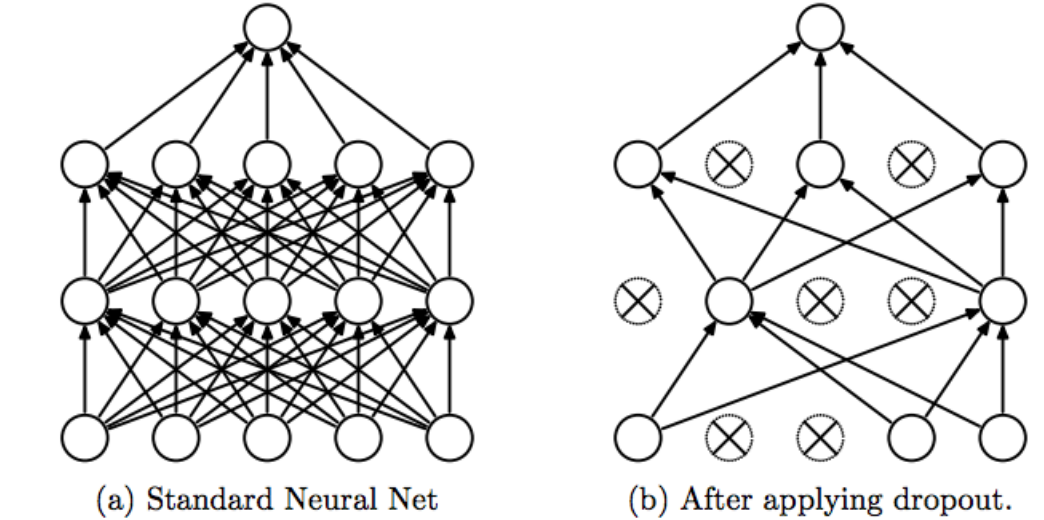
\includegraphics[width=0.9\textwidth]{figures/dro_out_lay.png}
	\caption{Drop-out layer \cite{dro_out_lay}}
	\label{fig:drop-out layer}
\end{figure}

\subsection{Softmax layer}
Ultimul strat dintr-o rețea neuronală convoluțională este un \textit{loss layer} folosing abordarea softmax.\newline
Acest strat are responsabilitatea de a calcula deviația dintre predicția rețelei și realitate (valoarea expectată). 


\label{cap:fund-teoretice}
\chapter{Prezentarea contribuțiilor autorului}
\label{cap:contributii}
În acest capitol se face prezentarea contribuțiilor autorului: un studiu comparativ a metodelor existente de detecția obiectelor și segmentarea semantică a imaginilor bazate pe rețele neuronale convoluționale.\newline
Se vor analiza în detaliu algoritmii care au la bază inteligență artificială deorece performanța acestora în domeniul prelucrării imaginilor depășește semnificativ orice altă metodă (algoritmi de nivel mai jos, cum ar fi algoritmii de thresholding) datorită faptului că rețelele neuronale nu sunt influențate de zgomotul din imagini, dar și pentru că sunt capabile de a produce rezultate în timp real \cite{cat_amz}.


\section{Categorii de algoritmi de segmentarea imaginilor}
Segmentarea imaginilor este unul dintre cele mai importante procese în domeniul viziunii artificiale moderne. Segmentarea imaginilor înseamnă etichetarea fiecărui pixel, ca aparținând unui obiect din imagine. Segmentele rezultate corespund unităților structurale (obiecte) din scenă. Segmentarea imaginilor este o problemă dificilă, pentru că nu există un model matematic care ar putea descrie bine procesul \cite{cat_amz}.\newline
Există un număr mare de algoritmi propuse în literatură, care vor fi prezentate în acest capitol. Favorizarea unei metode depinde numai de situație și de tipul de imagine care trebuie segmentat. Nu există nicio metodă universală, care produce rezultate bune pe fiecare tip de imagine. Chiar și alegerea metodei corespunzătoare pentru un tip de imagine este o problemă dificilă. Metode dezvoltate pentru un tip de imagine pot produce rezultate proaste pe alt tip de imagine.\newline
Technicile de segmentare pot fi plasate în trei clase mai mari:
\begin{itemize}
	\item algoritmi clasici bazate pe matematică sau metode statistice
	\item technici bazate pe inteligență artificială
	\item alte technici care fie sunt metode hibride, fie nu moștenesc din nicio categorie
\end{itemize}

Algoritmii clasici includ detecția marginilor obiectelor(\textit{edge/boundary detection)}, methode de thresholding (\textit{characteristic histogram thresholding)}, extragerea regiunilor (\textit{region extraction/region growing)} și abordări semantice și sintactice.\newline
Metodele de segmentare din domeniul inteligenței artificiale sunt de regulă metode care folosesc rețele neuronale.\newline

\subsection{Technici Bazate pe Rețele Neuronale Artificiale}
Începând cu anii 1990, rețelele neuronale au apărut și în domeniul prelucrării imaginilor și a viziunii artificiale. Având capabilități dorite (e.g. sunt insensibile la zgomotul din imagini, pot funcționa în timp real) au devenit foarte populare. Bineînțeles, diferite rețele neuronale au fost aplicate cu diferite nivele de succes; rețelele feed-forward back-propagation s-au dovedit a fi cele mai efective.\newline
Rețelele neuronale capabile de segmentare semantică pot fi împărțite în două categorii: rețele supravegheate și rețele nesupravegheate. Rețelele supravegheate au nevoie de set de antrenare etichetată, adică imagini pe care regiunile de interes sunt notate, având la îndemână și tipul obiectelor din zonele respective. Metodele nesupravegheate (numite și \textit{clustering processes}) sunt semi- sau total automate.

\subsubsection{Rețele supravegheate}
Rețelele neuronale care sunt antrenare cu învățare supravegheată au nevoie de un operator uman pentru a alege imaginile de antrenare și pentru a le segmenta în \textit{k} regiuni, fiecare fiind etichetat (cu tipul obiectului în regiune). Architectura propusă este antrenată folosind imaginile etichetate ca set de antrenare. După antrenare, rețeaua neuronală va fi capabilă de a segmenta imagini similare, asignând etichete pentru regiuni folosind cunoștințele acumulate la faza de antrenare.

\subsection{Detecția și Localizarea Obiectelor}
Este o confuzie generală între clasificarea imaginilor și detecția obiectelor din scene. Clasificarea imaginilor (\textit{image classification}) constă în obținerea unei predicții la ieșirea unui sistem referitor la tipul de obiect care era plasat în imaginea de intrare. Pe de altă parte, dacă vrem să identificăm locația obiectelor într-o imagine, și de exemplu să le numărăm numărul instanțelor unui obiect, putem folosi algoritmi de detecția obiectelor (\textit{object detection and localization}).\newline
%IoU Intersect over Union
\begin{figure}[h!]
    	\centering
	\captionsetup{justification=centering, margin=2cm}
	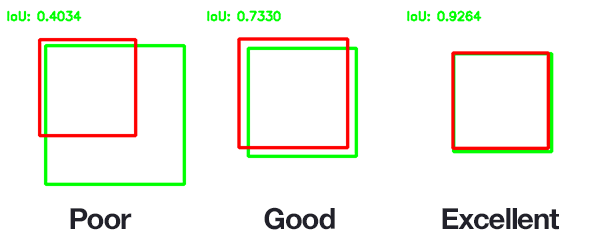
\includegraphics[width=0.5\textwidth]{figures/iou.png}
	\caption{Detecția obiectelor \cite{class_detect_segment}}
	\label{fig:class_detect_segment}
\end{figure}

\subsubsection{IoU - Intersect over Union}
Eficiența unui algoritm de localizare se măsoară folosind un algoritm de \textit{Intersect over Union}. Intersect over Union este o metodă pentru a evalua cât de aproape sunt predicțiile unui algoritm de detecția obiectelor de adevăr. \newline
Când vrem să măsurăm performanța rețelei antrenate, la stratul de intrare dăm imagini conținând obiecte care pot fi recunoscute și localizate de rețea, acesta specificând la stratul de ieșire predicția coordonatelor bounding-boxului fiecărui obiect. Aceste coordonate se compară cu cele reale, și se calculează Intersect over Union între dreptunghiurile definite de coordonatele specificate de rețea și dreptunghiurile reale (imaginile fiind etichetate avem la îndemână dreptunghiurile care conțin cu adevărat obiectele din imagini).
%object detection and localization
\begin{figure}[h!]
    	\centering
	\captionsetup{justification=centering, margin=2cm}
	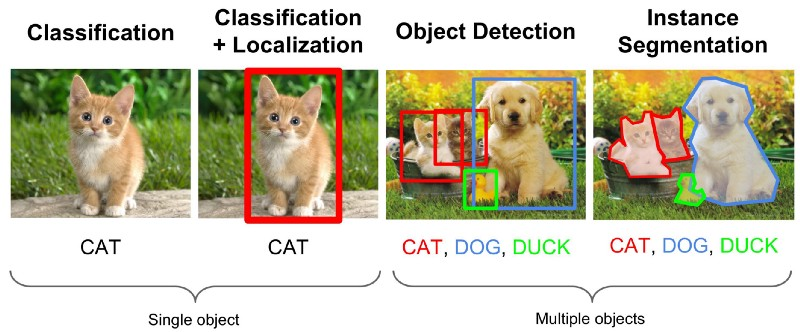
\includegraphics[width=0.9\textwidth]{figures/class_detect_segment.jpeg}
	\caption{Detecția obiectelor \cite{class_detect_segment}}
	\label{fig:class_detect_segment}
\end{figure}

\url{https://leonardoaraujosantos.gitbooks.io/artificial-inteligence/content/object_localization_and_detection.html}
\url{https://medium.com/nanonets/how-to-do-image-segmentation-using-deep-learning-c673cc5862ef}
Cinci abordări pentru detecția și localizarea obiectelor vor fi analizate și comparate:
\begin{itemize}
	\item RCNN
	\item Fast RCNN
	\item Faster RCNN
	\item Yolo
	\item SSD
\end{itemize}

\subsubsection{RCNN}
\url{https://towardsdatascience.com/r-cnn-fast-r-cnn-faster-r-cnn-yolo-object-detection-algorithms-36d53571365e}
Când se face detectarea obiectelor o problemă cu care ne întâlnim inevitabil este faptul că în majoritatea cazurilor nu o să fie numai un bounding box pentru o scenă pentru că imaginea respectivă poate să conțină numeroase obiecte de interes și nu putem să știm dinainte câte. Din acest motiv nu putem să folosim o rețea neuronală standard extinsă cu un strat fully connected.\newline
RCNN (Regions + CNN) este o metodă care se bazează pe o metodă externă de propunere de regiuni care găsește regiunile de interes, și le găsește repede. Algoritmul extern de propunere de regiuni se numește \textit{selective search}.\newline
Chiar și accelerând pasul de generare de regiuni de interes, problema cu RCNN este că nu este destul de rapid.\newline
Cu ajutorul selective search se generează 2000 de regiuni cu potențial mare de a conține vreun obiect de interes. Regiunile generate de selective search sunt numite propuneri de regiuni (\textit{region proposals}). Aceste propuneri de regiuni sunt introduse într-o rețea convoluțională care produce un vector de trăsături. Astfel rețeaua convoluțională funcționează ca un extractor de trăsături, iar stratul de ieșire conține trăsăturile extrase care sunt introduse într-un support vector machine pentru a clasifica prezența unui obiect în propunerea de regiune.\newline
RCNN are și câteva dezavantaje:
\begin{itemize}
	\item chiar și cu accelerarea pasului de propunere de regiuni timpul de antrenare a rețelei este lung, pentru că pentru fiecare imagine este nevoie de clasificarea a 2000 de propuneri de regiuni
	\item nu poate funcționa în timp real, pentru că detectarea obiectelor durează 47 de secunde în medie pentru imagine
	\item algoritmul selective search nu poate fi îmbunătățit, nici nu poate să învețe. Asta poate duce la generarea neadecvată a propunerilor de regiuni.
\end{itemize}

\subsubsection{Fast RCNN}
\url{https://towardsdatascience.com/r-cnn-fast-r-cnn-faster-r-cnn-yolo-object-detection-algorithms-36d53571365e}
Autorii articolului de RCNN au rezolvat câteva din problemele modelului RCNN pentru a construi un algoritm mai rapid pentru detectarea obiectelor. Acest algoritm îmbunătăți se numește Fast RCNN și este similar cu RCNN. Însă în loc de introducerea propunerilor de regiuni într-un CNN, se introduc imaginile în CNN pentru a genera o hartă de trăsături extrase cu o rețea convoluțională. Din această mapă identificăm propunerile de regiuni și folosim un strat softmax pentru a produce predicții de clasificare pentru regiuni.\newline
Fast RCNN este mai rapid decât predecesorul lui pentru că nu trebuie să introducem 2000 propuneri de regiuni în rețeaua convoluțională de fiecare dată; în schimb operația de convoluție se face o dată per imagine, pentru a genera harta trăsăturilor convoluționale.

%RCNN vs Fast RCNN training and testing times
\begin{figure}[h!]
    	\centering
	\captionsetup{justification=centering, margin=2cm}
	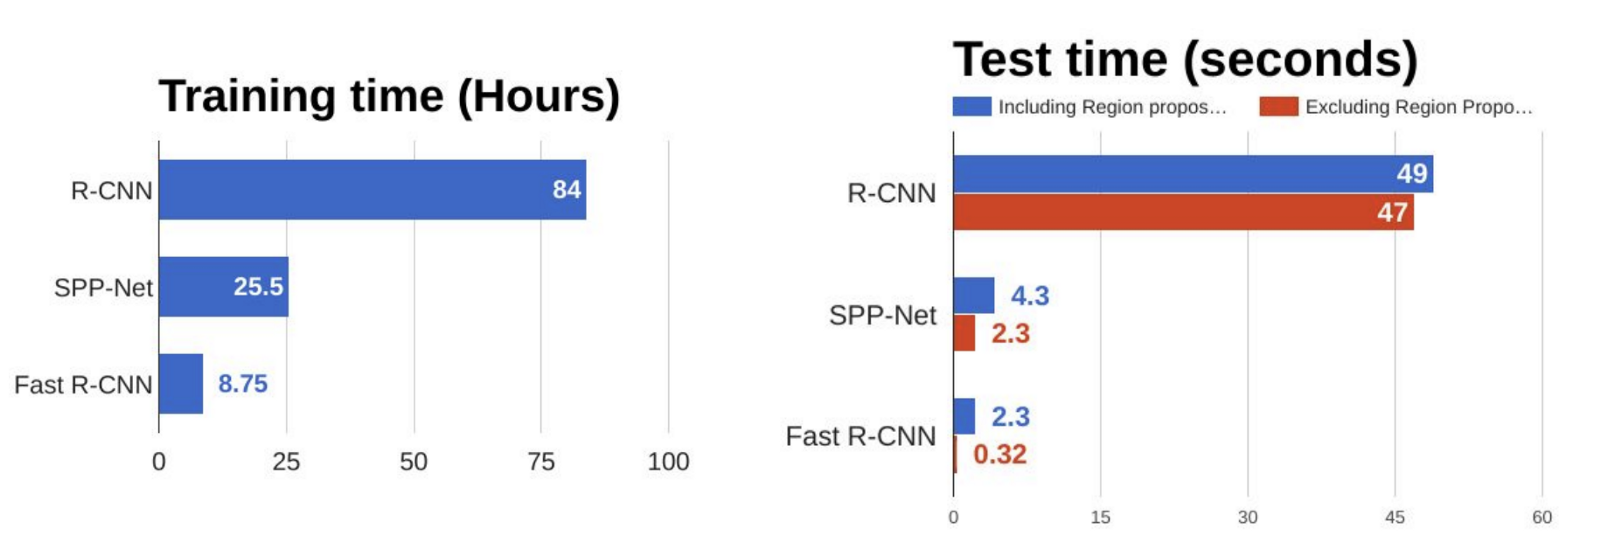
\includegraphics[width=0.9\textwidth]{figures/rcnn_vs_fast_rcnn_time.png}
	\caption{Diferența semnificativă dintre timpul de antrenare și testare între RCNN și Fast RCNN \cite{rcnn_vs_fast_rcnn}}
	\label{fig:class_detect_segment}
\end{figure}
Din acest grafic putem vedea că diferența dintre vitezele a rețelelor este semnificativă. Când ne uităm la performanța rețelei Fast RCNN observăm că performanța lui este mult mai bună fără folosirea metodei de propunere de regiuni. Deci algoritmul de propunere de regiuni este un bottleneck pentru Fast RCNN, afectând semnificativ performanța.

\subsubsection{Faster RCNN}
Ambii algoritmi de mai sus (RCNN și Fast RCNN) folosesc algoritmul selective search pentru a găsi propuneri de regiuni - regiuni cu potențial mare de a conține vreun obiect de interes. Acest algoritm este unul lent, consumă mult timp deci afectează performanța rețelei.\newline
Faster RCNN este similar cu Fast RCNN privind că și aici din imaginea introdusă se generează o hartă de trăsături convoluționale. În schimb aici nu se folosește selective search pentru a găsi regiunile de interes în harta de trăsături; în loc de acesta, o rețea separată este antrenată pentru a găsi predicții pentru coordonaterle regiunilor de interes. Regiunile previzionate sunt remodelate cu un strat RoI pooling și rezultatul este clasificat.

%RCNN vs Fast RCNN vs Faster RCNN testing time
\begin{figure}[h!]
    	\centering
	\captionsetup{justification=centering, margin=2cm}
	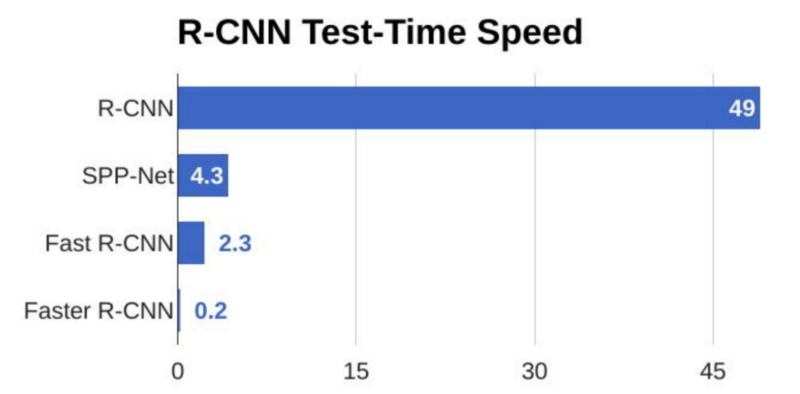
\includegraphics[width=0.8\textwidth]{figures/faster_rcnn_speed.png}
	\caption{Diferența dintre timpul de testare între  Fast RCNN și  Faster RCNN \cite{rcnn_vs_fast_rcnn}}
	\label{fig:class_detect_segment}
\end{figure}
Se vede că Faster RCNN este mult mai rapid decât predecesorii săi. Deja se poate folosi și pentru detectare de obiecte în timp real.\newline
Rețelele detaliate până aici au o trăsătură în comun: au o parte a rețelei dedicată pentru propunerea de regiuni, urmată de un clasificator performant. Aceste metode sunt capabile de o precizie ridicată, dar au dezavantajul că funcționează foarte lent (low frame-rate), însemnând că nu pot folosite în dispozitive embedded.\newline
O altă modalitate de a face detectare de obiecte este combinarea celor două pași (propuneri de regiuni și clasificare) într-o singură rețea. Acest scop poate fi atins cu o rețea care are un set predefinit de regiuni pentru găsirea obiectelor.\newline
O metodă pentru a refolosi rezultatul calculelor deja făcute la pasul de clasificare pentru localizare de obiecte este de a lua activările de la ultimul strat convoluțional. Aici încă avem informație spațială dar reprezentată într-o versiune mai mică decât în imaginea originală. De exemplu o imagine de 640x480x3 încărcată la stratul de intrare, pe ultimul strat convoluțional poate să producă ieșirea de dimensiunile 13x18x2048.\newline
Deci pe ultimul strat fiecare "pixel" reprezintă o zonă mai mare a imaginii de intrare, deci putem folosi aceste celule pentru a deduce poziția obiectelor.

%"pixels" from last layer correspond to larger areas on the original image
\begin{figure}[h!]
    	\centering
	\captionsetup{justification=centering, margin=2cm}
	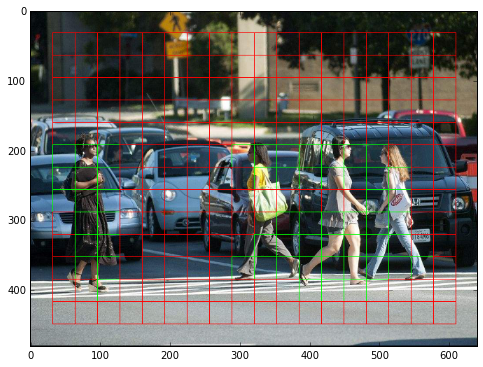
\includegraphics[width=0.8\textwidth]{figures/last_con_lay_to_inp_img.png}
	\caption{Diferența dintre timpul de testare între  Fast RCNN și  Faster RCNN \cite{rcnn_vs_fast_rcnn}}
	\label{fig:class_detect_segment}
\end{figure}

Un detaliu la care trebuie să fim atenți este că la folosirea fiecărui strat de pooling, pierdem o porțiune semnificativă de informație spațială.\newline
La acest pas putem folosi un strat convoluțional de 1x1 pentru a efectua o clasificare a fiecărei celule (e.g. pieton sau fundal), dar putem atașa încă un strat convoluțional sau fully-connected pentru a afla o predicție pentru cele 4 numere care descriu un bounding-box pentru obiectul conținut în celulă. Astfel primim clasificarea obiectului din regiune dar și locația sa.\newline
Este greșit să ne gândim ca și imaginea de intrare ar fi împărțită în celule înaintea începerii algoritmului. Ce se întâmplă de fapt este că fiecare strat reprezintă imaginea de intrare cu rezoluție mai mică, dar adâncime crescătoare. La antrenare facem a reconciliere între eticheta predefinită a imaginii și celulele virtuale (celulele pot să se suprapună).\newline
Familia detectoarelor de obiecte care folosesc această strategie:
\begin{itemize}
	\item SSD: folosește diferite matrice de activare (\textit{activation map}) pentru predicția claselor și a regiunilor
	\item YOLO: foloseste o singură matrice de activare pentru ambiele sarcini
	\item R-FCN (Region based Fully-Convolutional Neural Networks): funcționează mai rapid decât metodele (R-CNN, Fast R-CNN, etc) pentru că face puține calcule per celulă și este fully-conbolutional (conține numai straturi convoluționale).
\end{itemize}
Strategia acestor metode:
\begin{enumerate}
	\item se antrenează un CN cu regresiune (pentru bounding box) și clasificare (cu loss function)
	\item de obicei funcțiile de eroare sunt mai complexe pentru că trebuie să se descurce cu mai multe obiective (clasificare, regresiune, verificarea existenței unui obiect, etc.)
	\item culegerea activărilor de la un strat particular pentru a fi capabil de clasificare și localizare cu un strat FC sau un alt strat convoluțional
	 \item la pasul de prediction se folosesc algoritmi ca și \textit{non-maxima suppression} pentru a filtra multiple regiuni în jurul aceluiași obiect
	\item la stagiul de antrenare se folosesc algoritmi precum IoU (\textit{Intersect over Union}) pentru a afla corectitudinea localizării obiectului.
\end{enumerate}


\subsubsection{YOLO - You Only Look Once}
Până aici fiecare algoritm folosește regini pentru a localiza obiectele de interes în imagine. În loc să se uită la imaginea întreagă, rețeaua încearcă să găsească obiecte în părți care au potențial mare de a conține vreun obiect de interes.\newline
YOLO sau You Only Look Once este un algoritm de detectare de obiecte foarte diferit de algoritmii pe care le-am văzut până acum, fiindcă o singură rețea convoluțională este folosit atât pentru predicția bounding boxurilor cât și pentru clasificarea obiectelor din acestea.\newline
Acest detector are o precizie un pic mai mică dar funcționează foarte rapid (este capabil de detectare în timp real).

%YOLO functioning #1
\begin{figure}[h!]
    	\centering
	\captionsetup{justification=centering, margin=2cm}
	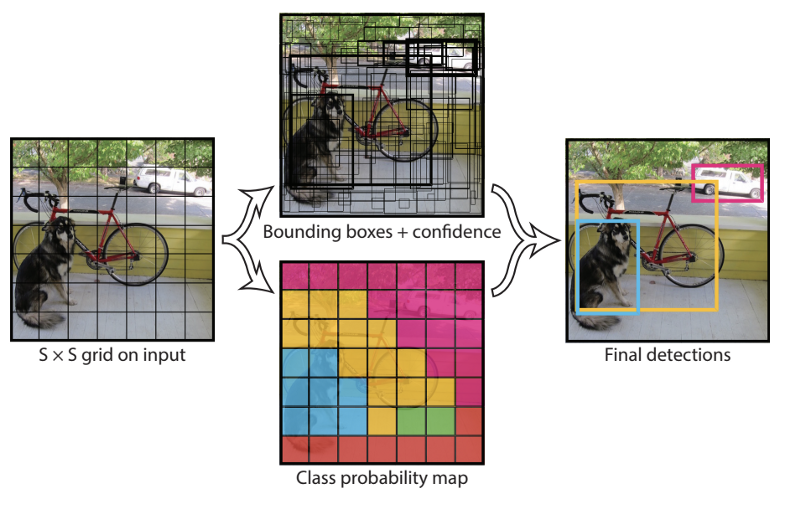
\includegraphics[width=0.8\textwidth]{figures/yolo1.png}
	\caption{YOLO \cite{rcnn_vs_fast_rcnn}}
	\label{fig:class_detect_segment}
\end{figure}

\paragraph{Ideea Principală}
Ideea din spatele acestui detector este că rulăm fiecare imagine printr-un model CNN și primim bounding boxes pentru obiecte într-un singur pas. Prima dată imaginea este redimensionată la rezoluția de 448x448, apoi încărcată în rețea. Ieșirea rețelei este filterată de un algoritm \textit{non-max suppression}.
Ieșirea modelului este un tensor batch de dimensiunile 7x7x30, și următorarele informații sunt codificate:
\begin{itemize}
	\item 2 definiții de bounding box: numere care identifică dreptungiul în care se află obiectul de interes (x, y, lățime, înălțime)
	\item 20 de probabilități de clase
\end{itemize}
Rețeaua este compuse folosind 9 straturi convoluționale, iar după ultimul strat de max-pool, din imaginea originală de 448x448 obținem o imagine de 7x7.\newline
Această ieșire de 7x7 poate fi considerată ca un grid de 7x7 reprezentând imaginea originală, unde fiecare celulă are 2 definiții de bounding box și 20 de probabilități de clase (celulele având o probabilitate de să aparțină unei clase din cele 20). Putem observa că această informație ne ajută și la detectarea clasei de obiect în care aparține entitatea din celulele respective.

%YOLO grid with possibilities
\begin{figure}[h!]
    	\centering
	\captionsetup{justification=centering, margin=2cm}
	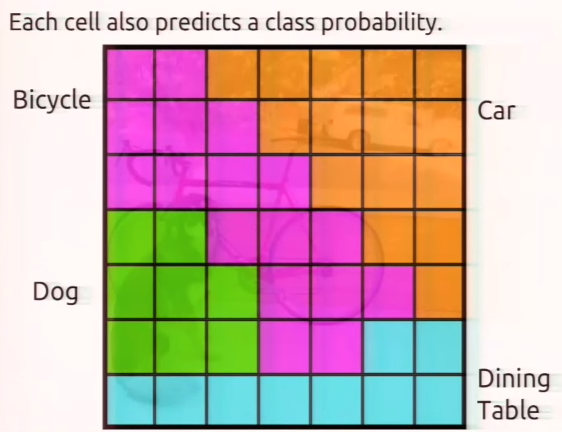
\includegraphics[width=0.7\textwidth]{figures/yolo_cell_class.png}
	\caption{YOLO \cite{rcnn_vs_fast_rcnn}}
	\label{fig:class_detect_segment}
\end{figure}

În ultimul pas folosind \textit{thresholding} și \textit{non-maxima suppression} putem filtra regiunile care nu sunt detectări valide.


More about YOLO if needed only
\url{https://leonardoaraujosantos.gitbooks.io/artificial-inteligence/content/single-shot-detectors/yolo.html}

\subsubsection{Multibox Single Shot Detector (SSD)}	






Titlul acestui capitol nu este unul impus și nici nu corespunde neapărat unui singur capitol. Titlul indică mai degrabă o parte (importantă și centrală, de altfel) a lucrării, în care se prezintă ceea ce s-a realizat efectiv: contribuțiile autorului. Organizarea acestei părți este dependentă și specifică fiecărei lucrări în parte și este stabilită de către fiecare autor după cum i se pare mai potrivit pentru tema lui. Ea poate cuprinde prezentarea unor concepte teoretice (unelte sau tehnici matematice folosite în lucrare, prezentarea sau introducerea unor concepte teoretice etc.), o analiză a diferitelor metode/algoritmi/tehnologii etc. luate în considerare sau dezvoltate de către autor, o prezentare a unui design (mai mult sau mai puțin detaliat) sau chiar detalii a unei eventuale implementări/prototip, dacă e cazul.

Trebuie remarcat însă faptul că această parte reprezintă contribuția personală a autorului, chiar dacă ea constă de exemplu doar dintr-o analiză comparativă a unor metode/algoritmi, și în nici un caz ea nu poate fi sinteza unor texte preluate din alte surse. Prin urmare, orice informații sunt prezentate aici, ele trebuie să corespundă cel puțin unei interpretări/analize critice personale a autorului, dacă nu chiar unor idei originale ale acestuia. 

\subsection{Dimensiune}

Împreună cu capitolul (partea) următor reprezintă cca. 70\% din lucrare. 


\section{Examples: lists, figures, tables, equations}

Așa arată o listă de elemente nenumerotate:
\begin{itemize}
  \item element 1
  \item element 2
  \item \dots
\end{itemize}


Așa arată o listă de elemente numerotare:
\begin{itemize}
  \item element 1
  \item element 2
  \item \dots
\end{itemize}


Așa arată o listă în text: 
\begin{inparaenum}[(\itshape 1 \upshape)]
  \item element 1, 
  \item element 2, 
  \item \dots
\end{inparaenum}

\textbf{Atenție}: orice tabel, figura sau ecuație (formulă) trebuie referite \textit{explicit} în text explicit (de genul: în Figura X este ulustrat \dots, în Tabelul Y se poate vedea \dots), pentru că Latex le poate plasa chiar și pe altă pagină decât acolo unde vrem noi să ne referim la ele. Vedeți exemple de mai jos!

Tabelul~\ref{table:example} ilustrează un exemplu de tabel. Un editor on-line de tabele poate fi găsit la \url{http://www.tablesgenerator.com/}. 

\begin{table}[t]
\centering                          % tabel centrat 
\begin{tabular}{|c|c|c|c|}          % 4 coloane centrate 
\hline\hline                        % linie orizontala dubla
Case & Method\#1 & Method\#2 & Method\#3 \\ [0.5ex]   % inserare tabel
%heading
\hline                              % linie orizontal simpla
1 & 50 & 837 & 970 \\               % corpul tabelului 
2 & 47 & 877 & 230 \\
3 & 31 & 25 & 415 \\[1ex]           % [1ex] adds vertical space
\hline                              
\end{tabular}
\caption{Nonlinear Model Results}   % titlul tabelului
\label{table:example}                % \label{table:nonlin} introduce eticheta folosita pentru referirea tabelului in text; referirea in text se va face cu \ref{table:nonlin}
\end{table}

În Figura~\ref{fig:exemplu} 

\begin{figure}
    \centering
    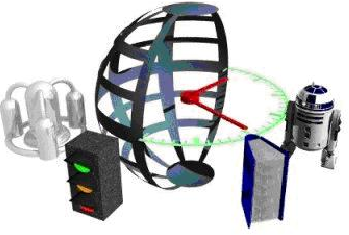
\includegraphics[width=0.5\textwidth]{image}
    \caption{Numele figurii}
    \label{fig:exemplu}
\end{figure}


Formula~(\ref{eq:example}) arată modul de calcul al lui $\Delta$:
\begin{equation} \label{eq:example}
    \Delta =\sum_{i=1}^N w_i (x_i - \bar{x})^2 .
\end{equation}


Algoritmul~\ref{alg:example} este un exemplu de descriere pseudo-cod a unui algoritm, preluat de la \href{http://en.wikibooks.org/wiki/LaTeX/Algorithms#Typesetting_using_the_algorithm2e_package}{http://en.wikibooks.org/wiki/LaTeX}. El utilizează pachetul \textit{algorithm2e}. Alternativ, puteți utiliza pachetele \textit{algorithmic} sau \textit{program}. 

\begin{algorithm}
 \KwData{this text}
 \KwResult{how to write algorithm with \LaTeX2e }
 initialization\;
 \While{not at end of this document}{
  read current\;
  \eIf{understand}{
   go to next section\;
   current section becomes this one\;
   }{
   go back to the beginning of current section\;
  }
 }
 \caption{How to write algorithms}
 \label{alg:example}
\end{algorithm}

% \chapter{Tests and Results}
\chapter{Rezultate teoretice și experimentale}
\label{cap:rezultate}
Comparația corectă a diferitelor algoritmi de segmentare semantică a imaginilor și de detecția obiectelor este o sarcină foarte grea; nu se poate stabili care dintre modele este cel mai bun. În aplicațiile din viața reală, alegerea modelului potrivit se face prin balansarea capabilităților ei: viteza de funcționare și acuratețe. Pe lângă alegerile referitoare la detector, câțiva alți factori trebuie luate în considerare când vorbim de comparație:

% enumerate shit which is crucial for making a good object detector
\begin{enumerate}
	\item rezoluția imaginii de intrare
	\item numărul propunerilor generate pentru a fi clasificate
	\item setul de antrenare
	\item extractorul de trăsături folosit
	\item funcția de cost pentru antrenare de localizare
	\item configurarea antrenării (viteza de antrenare a rețelei neuronale, mărimea loturilor de antrenare, micșorarea ratei de învățare)
	\item etc.
\end{enumerate}

Mai rău, technologia evoluează atât de repede încât orice comparație devine încechită destul de repede.\newline
În această parte a lucrării sumarizăm rezultatele din articole individuale, pentru a arăta imaginea de ansamblu a algoritmilor.

\section{Rezultate de Performanță}
În această secțiune sumarizăm performanțele diferitelor modele raportate în articolele corespunzătoare.\newline
Metrica pentru măsurarea performanței în contextul detecției obiectelor este \textit{mAP (mean Average Precision)}. Este definit ca \textit{the average of the maximum precisions at different recall values}, adică media maximelor precizii la diferite valori de rechemare. Pentru a înțelege acest concept, trebuie mai întâi să recapitulăm conceptele de precizie și rechemare mai întâi.
\paragraph{Precizie} măsoară acuratețea predicțiilor, i.e. procentul predicțiilor corecte.
\begin{equation}
Precizie = \frac{TruePositive}{TruePositive + FalsePositive}.
\end{equation}

\paragraph{Recall (rechemare)} măsoară cât de precise sunt identificările pozitive.
\begin{equation}
Recall = \frac{TruePositive}{TruePositive + FalsNegative}.
\end{equation}

\paragraph{AP} \textit{Average Precision} este media a mai multor IoU pentru toate categoriile de obiecte.

Următorul tabel prezintă preciziile diferitelor rețele de detectare de obiecte:

\begin{center}
    \begin{tabular}{| l | l | l | l |}
    \hline
    Method & mAP (\%) \\ \hline
    Fast R-CNN & 75.9 \\ \hline
    Faster R-CNN & 75.9 \\ \hline
    R-FCN & 82.0  \\ \hline
    SSD & 81.6 \\  \hline
    YOLO & 66.4 \\  \hline
    \end{tabular}
\end{center}



\subsection{Faster R-CNN}






Împreună cu partea de prezentare a proiectului, trebuie să reprezinte aproximativ 70\% din lucrare. 

Aici sunt prezentate metodele de validare a soluțiilor/sistemului descris în capitolele anterioare, scenariile de testare a corectitudinii funcționale, a utilizabilității, performanței etc.   

Rezultatele testelor experimentale necesită, în general interpretări (dacă rezultatele obținute corespund așteptărilor, intuițiilor cititorului, de ce apar variații/excepții etc.) și comparații cu rezultatele altor metode similare. 

Sistemele de testare și testele propriu-zise trebuie descrise detaliat astfel încât să poată fi reproduse și de alții care poate vor să-și compare soluțiile lor cu a voastră (eventual, codul testelor poate fi pus în anexe). Dacă se poate alegeți pentru evaluarea sistemului vostru benchmark-uri (pachete de testare) dedicate, astfel încât comparația cu alte sisteme să poată fi făcută mai ușor. În plus, astfel de teste sunt mult mai complete și mai realiste decât cele dezvoltate de voi. Oricum, încercați ca testele efectuate să nu fie triviale, ci să acopere scenarii cât mai reale, mai complexe și mai relevante ale funcționării sistemului vostru. 

% \section{Functional Tests}
\section{Teste de funcționalitate}



% \section{Performance Tests}
\section{Teste de performanță}
% \chapter{Conclusions}
\chapter{Conluzii}
\label{cap:concluzii}


\subsection{Realizări}
S-a realizat prezentarea detaliată a rețelelor neuronale, acestea fiind cele mai capabile modele folosite în domeniul detectării obiectelor și segmentării semantice a imaginilor. Am văzut cum se comportă blocul de construcție a rețelei: \textit{neuronul}, și cum se construiește rețeaua alcătuită din neuroni care sunt organizate în straturi și au "legături'' ponderate. Metodele de învățare forward propagation și backwards propagation au fost prezentate.\newline
După aceasta am văzut cum funcționează rețelele neuronale specifice domeniului viziunii artificiale (straturile speciale a acestora fiind prezentate).\newline
S-a făcut prezentarea comparativă a diferitelor metode de detectare de obiecte, și am construit o rețea bazându-se pe modelul YOLO (You Only Look Once).


\subsection{Îmbunătățiri posibile}
Câteva îmbunătățiri ar putea fi aduse:
\begin{enumerate}
	\item pentru rețeaua dezvoltată s-ar putea implementa un algoritm mai bun de non-maximum suppression. Acest lucru ar îmbunătăți metoda de calculare a costului la faza de antrenare a rețelei, astfel rețeaua ar putea să-și ajusteze ponderile într-un mod care ar duce la acuratețe mai mare (IoU și mAP ar fi mai mari)
	\item o altă îmbunătățire ar fi să facem rețeaua noastră capabilă să facă detectare de obiecte pe un stream video (momentan fiind capabil de a încărca imagini dintr-un fișier)
\end{enumerate}
% \include{ch8}

%\addcontentsline {toc}{chapter}{Bibliography}
\bibliographystyle{IEEEtran}
\bibliography{thesis}%same file name as for .bib

\appendix

\chapter{Diverse anexe}


\chapter{Demonstrații matematice detaliate (dacă există)}


\chapter{Pseudo-cod sau cod (dacă există)}

% \begin{verbatim}
%  /** Maps are easy to use in Scala. */
% object Maps {
%   val colors = Map("red" -> 0xFF0000,
%                    "turquoise" -> 0x00FFFF,
%                    "black" -> 0x000000,
%                    "orange" -> 0xFF8040,
%                    "brown" -> 0x804000)
%   def main(args: Array[String]) {
%     for (name <- args) println(
%       colors.get(name) match {
%         case Some(code) =>
%           name + " has code: " + code
%         case None =>
%           "Unknown color: " + name
%       }
%     )
%   }
% }
% \end{verbatim}


\begin{lstlisting}
 /** Maps are easy to use in Scala. */
object Maps {
  val colors = Map("red" -> 0xFF0000,
                   "turquoise" -> 0x00FFFF,
                   "black" -> 0x000000,
                   "orange" -> 0xFF8040,
                   "brown" -> 0x804000)
  def main(args: Array[String]) {
    for (name <- args) println(
      colors.get(name) match {
        case Some(code) =>
          name + " has code: " + code
        case None =>
          "Unknown color: " + name
      }
    )
  }
}
\end{lstlisting}


\chapter{Articole publicate}



\end{document}
